% Options for packages loaded elsewhere
% Options for packages loaded elsewhere
\PassOptionsToPackage{unicode}{hyperref}
\PassOptionsToPackage{hyphens}{url}
\PassOptionsToPackage{dvipsnames,svgnames,x11names}{xcolor}
%
\documentclass[
  letterpaper,
  DIV=11,
  numbers=noendperiod]{scrartcl}
\usepackage{xcolor}
\usepackage{amsmath,amssymb}
\setcounter{secnumdepth}{-\maxdimen} % remove section numbering
\usepackage{iftex}
\ifPDFTeX
  \usepackage[T1]{fontenc}
  \usepackage[utf8]{inputenc}
  \usepackage{textcomp} % provide euro and other symbols
\else % if luatex or xetex
  \usepackage{unicode-math} % this also loads fontspec
  \defaultfontfeatures{Scale=MatchLowercase}
  \defaultfontfeatures[\rmfamily]{Ligatures=TeX,Scale=1}
\fi
\usepackage{lmodern}
\ifPDFTeX\else
  % xetex/luatex font selection
\fi
% Use upquote if available, for straight quotes in verbatim environments
\IfFileExists{upquote.sty}{\usepackage{upquote}}{}
\IfFileExists{microtype.sty}{% use microtype if available
  \usepackage[]{microtype}
  \UseMicrotypeSet[protrusion]{basicmath} % disable protrusion for tt fonts
}{}
\makeatletter
\@ifundefined{KOMAClassName}{% if non-KOMA class
  \IfFileExists{parskip.sty}{%
    \usepackage{parskip}
  }{% else
    \setlength{\parindent}{0pt}
    \setlength{\parskip}{6pt plus 2pt minus 1pt}}
}{% if KOMA class
  \KOMAoptions{parskip=half}}
\makeatother
% Make \paragraph and \subparagraph free-standing
\makeatletter
\ifx\paragraph\undefined\else
  \let\oldparagraph\paragraph
  \renewcommand{\paragraph}{
    \@ifstar
      \xxxParagraphStar
      \xxxParagraphNoStar
  }
  \newcommand{\xxxParagraphStar}[1]{\oldparagraph*{#1}\mbox{}}
  \newcommand{\xxxParagraphNoStar}[1]{\oldparagraph{#1}\mbox{}}
\fi
\ifx\subparagraph\undefined\else
  \let\oldsubparagraph\subparagraph
  \renewcommand{\subparagraph}{
    \@ifstar
      \xxxSubParagraphStar
      \xxxSubParagraphNoStar
  }
  \newcommand{\xxxSubParagraphStar}[1]{\oldsubparagraph*{#1}\mbox{}}
  \newcommand{\xxxSubParagraphNoStar}[1]{\oldsubparagraph{#1}\mbox{}}
\fi
\makeatother

\usepackage{color}
\usepackage{fancyvrb}
\newcommand{\VerbBar}{|}
\newcommand{\VERB}{\Verb[commandchars=\\\{\}]}
\DefineVerbatimEnvironment{Highlighting}{Verbatim}{commandchars=\\\{\}}
% Add ',fontsize=\small' for more characters per line
\usepackage{framed}
\definecolor{shadecolor}{RGB}{241,243,245}
\newenvironment{Shaded}{\begin{snugshade}}{\end{snugshade}}
\newcommand{\AlertTok}[1]{\textcolor[rgb]{0.68,0.00,0.00}{#1}}
\newcommand{\AnnotationTok}[1]{\textcolor[rgb]{0.37,0.37,0.37}{#1}}
\newcommand{\AttributeTok}[1]{\textcolor[rgb]{0.40,0.45,0.13}{#1}}
\newcommand{\BaseNTok}[1]{\textcolor[rgb]{0.68,0.00,0.00}{#1}}
\newcommand{\BuiltInTok}[1]{\textcolor[rgb]{0.00,0.23,0.31}{#1}}
\newcommand{\CharTok}[1]{\textcolor[rgb]{0.13,0.47,0.30}{#1}}
\newcommand{\CommentTok}[1]{\textcolor[rgb]{0.37,0.37,0.37}{#1}}
\newcommand{\CommentVarTok}[1]{\textcolor[rgb]{0.37,0.37,0.37}{\textit{#1}}}
\newcommand{\ConstantTok}[1]{\textcolor[rgb]{0.56,0.35,0.01}{#1}}
\newcommand{\ControlFlowTok}[1]{\textcolor[rgb]{0.00,0.23,0.31}{\textbf{#1}}}
\newcommand{\DataTypeTok}[1]{\textcolor[rgb]{0.68,0.00,0.00}{#1}}
\newcommand{\DecValTok}[1]{\textcolor[rgb]{0.68,0.00,0.00}{#1}}
\newcommand{\DocumentationTok}[1]{\textcolor[rgb]{0.37,0.37,0.37}{\textit{#1}}}
\newcommand{\ErrorTok}[1]{\textcolor[rgb]{0.68,0.00,0.00}{#1}}
\newcommand{\ExtensionTok}[1]{\textcolor[rgb]{0.00,0.23,0.31}{#1}}
\newcommand{\FloatTok}[1]{\textcolor[rgb]{0.68,0.00,0.00}{#1}}
\newcommand{\FunctionTok}[1]{\textcolor[rgb]{0.28,0.35,0.67}{#1}}
\newcommand{\ImportTok}[1]{\textcolor[rgb]{0.00,0.46,0.62}{#1}}
\newcommand{\InformationTok}[1]{\textcolor[rgb]{0.37,0.37,0.37}{#1}}
\newcommand{\KeywordTok}[1]{\textcolor[rgb]{0.00,0.23,0.31}{\textbf{#1}}}
\newcommand{\NormalTok}[1]{\textcolor[rgb]{0.00,0.23,0.31}{#1}}
\newcommand{\OperatorTok}[1]{\textcolor[rgb]{0.37,0.37,0.37}{#1}}
\newcommand{\OtherTok}[1]{\textcolor[rgb]{0.00,0.23,0.31}{#1}}
\newcommand{\PreprocessorTok}[1]{\textcolor[rgb]{0.68,0.00,0.00}{#1}}
\newcommand{\RegionMarkerTok}[1]{\textcolor[rgb]{0.00,0.23,0.31}{#1}}
\newcommand{\SpecialCharTok}[1]{\textcolor[rgb]{0.37,0.37,0.37}{#1}}
\newcommand{\SpecialStringTok}[1]{\textcolor[rgb]{0.13,0.47,0.30}{#1}}
\newcommand{\StringTok}[1]{\textcolor[rgb]{0.13,0.47,0.30}{#1}}
\newcommand{\VariableTok}[1]{\textcolor[rgb]{0.07,0.07,0.07}{#1}}
\newcommand{\VerbatimStringTok}[1]{\textcolor[rgb]{0.13,0.47,0.30}{#1}}
\newcommand{\WarningTok}[1]{\textcolor[rgb]{0.37,0.37,0.37}{\textit{#1}}}

\usepackage{longtable,booktabs,array}
\usepackage{calc} % for calculating minipage widths
% Correct order of tables after \paragraph or \subparagraph
\usepackage{etoolbox}
\makeatletter
\patchcmd\longtable{\par}{\if@noskipsec\mbox{}\fi\par}{}{}
\makeatother
% Allow footnotes in longtable head/foot
\IfFileExists{footnotehyper.sty}{\usepackage{footnotehyper}}{\usepackage{footnote}}
\makesavenoteenv{longtable}
\usepackage{graphicx}
\makeatletter
\newsavebox\pandoc@box
\newcommand*\pandocbounded[1]{% scales image to fit in text height/width
  \sbox\pandoc@box{#1}%
  \Gscale@div\@tempa{\textheight}{\dimexpr\ht\pandoc@box+\dp\pandoc@box\relax}%
  \Gscale@div\@tempb{\linewidth}{\wd\pandoc@box}%
  \ifdim\@tempb\p@<\@tempa\p@\let\@tempa\@tempb\fi% select the smaller of both
  \ifdim\@tempa\p@<\p@\scalebox{\@tempa}{\usebox\pandoc@box}%
  \else\usebox{\pandoc@box}%
  \fi%
}
% Set default figure placement to htbp
\def\fps@figure{htbp}
\makeatother





\setlength{\emergencystretch}{3em} % prevent overfull lines

\providecommand{\tightlist}{%
  \setlength{\itemsep}{0pt}\setlength{\parskip}{0pt}}



 


\usepackage{float}
\usepackage{tabularray}
\usepackage[normalem]{ulem}
\usepackage{graphicx}
\usepackage{rotating}
\UseTblrLibrary{siunitx}
\NewTableCommand{\tinytableDefineColor}[3]{\definecolor{#1}{#2}{#3}}
\newcommand{\tinytableTabularrayUnderline}[1]{\underline{#1}}
\newcommand{\tinytableTabularrayStrikeout}[1]{\sout{#1}}
\KOMAoption{captions}{tableheading}
\makeatletter
\@ifpackageloaded{caption}{}{\usepackage{caption}}
\AtBeginDocument{%
\ifdefined\contentsname
  \renewcommand*\contentsname{Table of contents}
\else
  \newcommand\contentsname{Table of contents}
\fi
\ifdefined\listfigurename
  \renewcommand*\listfigurename{List of Figures}
\else
  \newcommand\listfigurename{List of Figures}
\fi
\ifdefined\listtablename
  \renewcommand*\listtablename{List of Tables}
\else
  \newcommand\listtablename{List of Tables}
\fi
\ifdefined\figurename
  \renewcommand*\figurename{Figure}
\else
  \newcommand\figurename{Figure}
\fi
\ifdefined\tablename
  \renewcommand*\tablename{Table}
\else
  \newcommand\tablename{Table}
\fi
}
\@ifpackageloaded{float}{}{\usepackage{float}}
\floatstyle{ruled}
\@ifundefined{c@chapter}{\newfloat{codelisting}{h}{lop}}{\newfloat{codelisting}{h}{lop}[chapter]}
\floatname{codelisting}{Listing}
\newcommand*\listoflistings{\listof{codelisting}{List of Listings}}
\makeatother
\makeatletter
\makeatother
\makeatletter
\@ifpackageloaded{caption}{}{\usepackage{caption}}
\@ifpackageloaded{subcaption}{}{\usepackage{subcaption}}
\makeatother
\usepackage{bookmark}
\IfFileExists{xurl.sty}{\usepackage{xurl}}{} % add URL line breaks if available
\urlstyle{same}
\hypersetup{
  pdftitle={final\_analysis},
  colorlinks=true,
  linkcolor={blue},
  filecolor={Maroon},
  citecolor={Blue},
  urlcolor={Blue},
  pdfcreator={LaTeX via pandoc}}


\title{final\_analysis}
\author{}
\date{}
\begin{document}
\maketitle


\begin{Shaded}
\begin{Highlighting}[]
\NormalTok{LIKERTS }\OtherTok{\textless{}{-}} \FunctionTok{c}\NormalTok{(}
  \CommentTok{\# English}
  \StringTok{"strongly disagree"}                         \OtherTok{=} \DecValTok{1}\NormalTok{L,}
  \StringTok{"disagree"}                                  \OtherTok{=} \DecValTok{2}\NormalTok{L,}
  \StringTok{"neutral"}                                   \OtherTok{=} \DecValTok{3}\NormalTok{L,}
  \StringTok{"agree"}                                     \OtherTok{=} \DecValTok{4}\NormalTok{L,}
  \StringTok{"strongly agree"}                            \OtherTok{=} \DecValTok{5}\NormalTok{L,}
  \CommentTok{\# Polish variants}
  \StringTok{"zdecydowanie nie zgadzam się"}              \OtherTok{=} \DecValTok{1}\NormalTok{L,}
  \StringTok{"zdecydowanie się nie zgadzam"}              \OtherTok{=} \DecValTok{1}\NormalTok{L,}
  \StringTok{"nie zgadzam się"}                           \OtherTok{=} \DecValTok{2}\NormalTok{L,}
  \StringTok{"raczej się nie zgadzam"}                    \OtherTok{=} \DecValTok{2}\NormalTok{L,}
  \StringTok{"neutralny"}                                 \OtherTok{=} \DecValTok{3}\NormalTok{L,}
  \StringTok{"nie mam opinii"}                            \OtherTok{=} \DecValTok{3}\NormalTok{L,}
  \StringTok{"ani się zgadzam, ani się nie zgadzam"}      \OtherTok{=} \DecValTok{3}\NormalTok{L,}
  \StringTok{"ani się zgadzam, ani nie"}                  \OtherTok{=} \DecValTok{3}\NormalTok{L,}
  \StringTok{"zgadzam się"}                               \OtherTok{=} \DecValTok{4}\NormalTok{L,}
  \StringTok{"raczej się zgadzam"}                        \OtherTok{=} \DecValTok{4}\NormalTok{L,}
  \StringTok{"zdecydowanie zgadzam się"}                  \OtherTok{=} \DecValTok{5}\NormalTok{L,}
  \StringTok{"zdecydowanie się zgadzam"}                  \OtherTok{=} \DecValTok{5}\NormalTok{L}
\NormalTok{)}

\CommentTok{\# ── 1.2  Purchase frequency ───────────────────────────────────────────────────}

\NormalTok{PURCHASE\_FREQ }\OtherTok{\textless{}{-}} \FunctionTok{c}\NormalTok{(}
  \StringTok{"less than once a month / occasionally"}               \OtherTok{=} \DecValTok{1}\NormalTok{L,}
  \StringTok{"rzadziej niż raz w miesiącu / sporadycznie"}          \OtherTok{=} \DecValTok{1}\NormalTok{L,}
  \StringTok{"once a month"}                                        \OtherTok{=} \DecValTok{2}\NormalTok{L,}
  \StringTok{"raz w miesiącu"}                                      \OtherTok{=} \DecValTok{2}\NormalTok{L,}
  \StringTok{"2–3 times a month"}                                   \OtherTok{=} \DecValTok{3}\NormalTok{L,}
  \StringTok{"2{-}3 razy w miesiącu"}                                 \OtherTok{=} \DecValTok{3}\NormalTok{L,}
  \StringTok{"once a week"}                                         \OtherTok{=} \DecValTok{4}\NormalTok{L,}
  \StringTok{"raz w tygodniu"}                                      \OtherTok{=} \DecValTok{4}\NormalTok{L,}
  \StringTok{"a few times a week"}                                  \OtherTok{=} \DecValTok{5}\NormalTok{L,}
  \StringTok{"kilka razy w tygodniu"}                               \OtherTok{=} \DecValTok{5}\NormalTok{L,}
  \StringTok{"daily"}                                               \OtherTok{=} \DecValTok{6}\NormalTok{L,}
  \StringTok{"codziennie"}                                          \OtherTok{=} \DecValTok{6}\NormalTok{L}
\NormalTok{)}

\CommentTok{\# ── 1.3  Purchase intention (F1) ──────────────────────────────────────────────}

\NormalTok{F1\_INTENT }\OtherTok{\textless{}{-}} \FunctionTok{c}\NormalTok{(}
  \StringTok{"no, i intend to decrease it"}      \OtherTok{=} \DecValTok{1}\NormalTok{L,}
  \StringTok{"i\textquotesingle{}m not sure"}                     \OtherTok{=} \DecValTok{2}\NormalTok{L,}
  \StringTok{"no, i will maintain the same level"} \OtherTok{=} \DecValTok{3}\NormalTok{L,}
  \StringTok{"pozostanie na tym samym poziomie"} \OtherTok{=} \DecValTok{3}\NormalTok{L,}
  \StringTok{"yes, slightly"}                    \OtherTok{=} \DecValTok{4}\NormalTok{L,}
  \StringTok{"raczej tak"}                       \OtherTok{=} \DecValTok{4}\NormalTok{L,}
  \StringTok{"yes, significantly"}               \OtherTok{=} \DecValTok{5}\NormalTok{L,}
  \StringTok{"zdecydowanie tak"}                 \OtherTok{=} \DecValTok{5}\NormalTok{L}
\NormalTok{)}



\CommentTok{\# ── 1.4  Certification logo familiarity ───────────────────────────────────────}

\NormalTok{CERT\_FAM }\OtherTok{\textless{}{-}} \FunctionTok{c}\NormalTok{(}
  \StringTok{"i do not recognize this logo at all"}              \OtherTok{=} \DecValTok{1}\NormalTok{L,}
  \StringTok{"nie, nie rozpoznaję tego logo"}                    \OtherTok{=} \DecValTok{1}\NormalTok{L,}
  \StringTok{"i have seen this logo but don\textquotesingle{}t know much about it"} \OtherTok{=} \DecValTok{2}\NormalTok{L,}
  \StringTok{"widziałem/am je, ale niewiele o nim wiem"}         \OtherTok{=} \DecValTok{2}\NormalTok{L,}
  \StringTok{"i recognize this logo and know what it means"}     \OtherTok{=} \DecValTok{3}\NormalTok{L,}
  \StringTok{"znam to logo i wiem, co oznacza"}                  \OtherTok{=} \DecValTok{3}\NormalTok{L}
\NormalTok{)}




\CommentTok{\# ── 1.5  Certification / logo importance ─────────────────────────────────────}

\NormalTok{CERT\_IMP }\OtherTok{\textless{}{-}} \FunctionTok{c}\NormalTok{(}
  \StringTok{"not important {-} it doesn\textquotesingle{}t affect my purchasing decisions"} \OtherTok{=} \DecValTok{1}\NormalTok{L,}
  \StringTok{"nieważne {-} nie wpływa na moje decyzje zakupowe"}           \OtherTok{=} \DecValTok{1}\NormalTok{L,}
  \StringTok{"i don\textquotesingle{}t pay attention to certification logos"}             \OtherTok{=} \DecValTok{1}\NormalTok{L,}
  \StringTok{"nie zwracam uwagi na logo certyfikatów"}                   \OtherTok{=} \DecValTok{1}\NormalTok{L,}
  \StringTok{"somewhat important {-} it influences my choice, but i sometimes buy uncertified"} \OtherTok{=} \DecValTok{2}\NormalTok{L,}
  \StringTok{"dość ważne {-} wpływa na mój wybór, ale czasem kupuję produkty niecertyfikowane"} \OtherTok{=} \DecValTok{2}\NormalTok{L,}
  \StringTok{"very important {-} i look for it and usually only buy certified products"}         \OtherTok{=} \DecValTok{3}\NormalTok{L}
\NormalTok{)}



\CommentTok{\# ── 1.6  Household economic situation (SES proxy) ────────────────────────────}

\NormalTok{HOUSEHOLD\_ECON }\OtherTok{\textless{}{-}} \FunctionTok{c}\NormalTok{(}
  \StringTok{"poor"}         \OtherTok{=} \DecValTok{1}\NormalTok{L,}
  \StringTok{"fair/average"} \OtherTok{=} \DecValTok{2}\NormalTok{L,}
  \StringTok{"przeciętna"}   \OtherTok{=} \DecValTok{2}\NormalTok{L,}
  \StringTok{"good"}         \OtherTok{=} \DecValTok{3}\NormalTok{L,}
  \StringTok{"dobra"}        \OtherTok{=} \DecValTok{3}\NormalTok{L,}
  \StringTok{"bardzo dobra"} \OtherTok{=} \DecValTok{4}\NormalTok{L,}
  \StringTok{"very good"}    \OtherTok{=} \DecValTok{4}\NormalTok{L}
\NormalTok{)}


\CommentTok{\# ── 1.7  Employment status ────────────────────────────────────────────────────}

\CommentTok{\# EMPLOYMENT \textless{}{-} c(}
\CommentTok{\#   "Employed full{-}time"                        = 1L,}
\CommentTok{\#   "Praca na pełny etat"                       = 1L,}
\CommentTok{\#   "Employed part{-}time"                        = 2L,}
\CommentTok{\#   "Praca w niepełnym wymiarze czasu"          = 2L,}
\CommentTok{\#   "self{-}employed / Freelancer"                = 3L,}
\CommentTok{\#   "Unemployed"                                = 4L,}
\CommentTok{\#   "Bezrobotna/ny"                             = 4L,}
\CommentTok{\#   "Retired"                                   = 5L,}
\CommentTok{\#   "Student"                                   = 6L,}
\CommentTok{\#   "Homemaker"                                 = 7L,}
\CommentTok{\#   "Osoba prowadząca gospodarstwo domowe"      = 7L}
\CommentTok{\# )}

\NormalTok{EMPLOYMENT }\OtherTok{\textless{}{-}} \FunctionTok{c}\NormalTok{(}
  \StringTok{"employed full{-}time"}                   \OtherTok{=} \DecValTok{5}\NormalTok{L,}
  \StringTok{"praca na pełny etat"}                  \OtherTok{=} \DecValTok{5}\NormalTok{L,}
  \StringTok{"self{-}employed / freelancer"}           \OtherTok{=} \DecValTok{5}\NormalTok{L,}
  \StringTok{"employed part{-}time"}                   \OtherTok{=} \DecValTok{4}\NormalTok{L,}
  \StringTok{"praca w niepełnym wymiarze czasu"}     \OtherTok{=} \DecValTok{4}\NormalTok{L,}
  \StringTok{"student"}                              \OtherTok{=} \DecValTok{3}\NormalTok{L,}
  \StringTok{"homemaker"}                            \OtherTok{=} \DecValTok{3}\NormalTok{L,}
  \StringTok{"osoba prowadząca gospodarstwo domowe"} \OtherTok{=} \DecValTok{3}\NormalTok{L,}
  \StringTok{"retired"}                              \OtherTok{=} \DecValTok{3}\NormalTok{L,}
  \StringTok{"unemployed"}                           \OtherTok{=} \DecValTok{2}\NormalTok{L,}
  \StringTok{"bezrobotna/ny"}                        \OtherTok{=} \DecValTok{2}\NormalTok{L,}
  \StringTok{"NA"}                                   \OtherTok{=} \DecValTok{1}\NormalTok{L}
\NormalTok{)}





\CommentTok{\# ── 1.8  Education ────────────────────────────────────────────────────────────}

\NormalTok{EDUCATION }\OtherTok{\textless{}{-}} \FunctionTok{c}\NormalTok{(}
  \CommentTok{\# Level 1: Primary}
  \StringTok{"primary or Less"}                            \OtherTok{=} \DecValTok{1}\NormalTok{L,}
  \StringTok{"podstawowe"}                                 \OtherTok{=} \DecValTok{1}\NormalTok{L,}
  
  \CommentTok{\# Level 2: Vocational (Lower Secondary/Trade)}
  \StringTok{"szkoła zawodowa"}                            \OtherTok{=} \DecValTok{2}\NormalTok{L, }
  
  \CommentTok{\# Level 3: Secondary / High School}
  \StringTok{"secondary/high school"}                      \OtherTok{=} \DecValTok{3}\NormalTok{L,}
  \StringTok{"średnie / liceum / technikum"}               \OtherTok{=} \DecValTok{3}\NormalTok{L,}
  \StringTok{"technical/vocational training"}              \OtherTok{=} \DecValTok{3}\NormalTok{L, }\CommentTok{\# Technikum is often here}
  \StringTok{"college"}                                    \OtherTok{=} \DecValTok{3}\NormalTok{L,}
  
  \CommentTok{\# Level 4: Bachelor\textquotesingle{}s / Engineer}
  \StringTok{"bachelor\textquotesingle{}s degree"}                          \OtherTok{=} \DecValTok{4}\NormalTok{L,}
  \StringTok{"wykształcenie wyższe (licencjat/inżynier)"}  \OtherTok{=} \DecValTok{4}\NormalTok{L,}
  
  \CommentTok{\# Level 5: Master\textquotesingle{}s or PhD}
  \StringTok{"master\textquotesingle{}s degree or higher"}                  \OtherTok{=} \DecValTok{5}\NormalTok{L,}
  \StringTok{"postgraduate Degree (masters, phd)"}         \OtherTok{=} \DecValTok{5}\NormalTok{L,}
  \StringTok{"doctorate"}                                  \OtherTok{=} \DecValTok{5}\NormalTok{L,}
  \StringTok{"wykształcenie wyższe (magister lub wyższe)"} \OtherTok{=} \DecValTok{5}\NormalTok{L,}
  \StringTok{"magister lub wyższy"}                        \OtherTok{=} \DecValTok{5}\NormalTok{L}
\NormalTok{)}
\end{Highlighting}
\end{Shaded}

\begin{Shaded}
\begin{Highlighting}[]
\CommentTok{\# ── 1.9  Colour palette (reused in all plots) ─────────────────────────────────}

\NormalTok{COL\_COUNTRY }\OtherTok{\textless{}{-}} \FunctionTok{c}\NormalTok{(}\StringTok{"Poland"} \OtherTok{=} \StringTok{"\#e41a1c"}\NormalTok{, }\StringTok{"Zimbabwe"} \OtherTok{=} \StringTok{"\#377eb8"}\NormalTok{)}

\CommentTok{\# ── 2.1  Read raw Excel ───────────────────────────────────────────────────────}

\CommentTok{\# Update the path to point to your local copy of the Excel file.}

\NormalTok{raw }\OtherTok{\textless{}{-}}\NormalTok{ readxl}\SpecialCharTok{::}\FunctionTok{read\_excel}\NormalTok{(}
  \StringTok{"data/Consumer Behavior towards Organic Food Comparative Study\_ Poland vs Zimbabwe (Responses) (2) (1).xlsx"}
\NormalTok{)}
\end{Highlighting}
\end{Shaded}

\begin{Shaded}
\begin{Highlighting}[]
\CommentTok{\# ── 2.2  Bilingual column coalescing ─────────────────────────────────────────}

\CommentTok{\# For each construct the survey has parallel English + Polish columns.}

\CommentTok{\# coalesce() picks the first non{-}NA value, so bilingual responses map}

\CommentTok{\# to a single canonical column.}

\NormalTok{coalesce\_map }\OtherTok{\textless{}{-}} \FunctionTok{list}\NormalTok{(}
  \AttributeTok{consent =} \FunctionTok{c}\NormalTok{(}\StringTok{"Do you agree to participate in this study after reading the information above?"}\NormalTok{, }\StringTok{"Czy po zapoznaniu się z powyższymi informacjami wyraża Pan/Pani zgodę na udział w tym badaniu?"}\NormalTok{),}
  \AttributeTok{purchased\_last\_12m    =} \FunctionTok{c}\NormalTok{(}\StringTok{"A1. Have you purchased or consumed any organic food products in the last 12 months?"}\NormalTok{, }\StringTok{"  A1. Czy w ciągu ostatnich 12 miesięcy kupował (a) Pan/Pani lub spożywał(a) produkty ekologiczne?  "}\NormalTok{),}
  \AttributeTok{age =} \FunctionTok{c}\NormalTok{(}\StringTok{"A2. Age:"}\NormalTok{, }\StringTok{"A2. Wiek:"}\NormalTok{),}
  \AttributeTok{gender =} \FunctionTok{c}\NormalTok{(}\StringTok{"A3. Gender"}\NormalTok{, }\StringTok{"A3. Płeć:"}\NormalTok{),}
  \AttributeTok{education =} \FunctionTok{c}\NormalTok{(}\StringTok{"A4. Highest Educational Level Completed:"}\NormalTok{, }\StringTok{"A4. Najwyższy ukończony poziom wykształcenia:"}\NormalTok{),}
  \AttributeTok{household\_econ =} \FunctionTok{c}\NormalTok{(}\StringTok{"A5. How would you describe the economic situation of your household?"}\NormalTok{, }\StringTok{"A5. Jak ocenia Pani/Pan sytuację ekonomiczną swojego gospodarstwa domowego?"}\NormalTok{),}
  \AttributeTok{employment =} \FunctionTok{c}\NormalTok{(}\StringTok{"A6. Current Employment Status:"}\NormalTok{, }\StringTok{"A6. Obecny status zatrudnienia:"}\NormalTok{),}
  \AttributeTok{country =} \FunctionTok{c}\NormalTok{(}\StringTok{"A7. Country of Residence:"}\NormalTok{, }\StringTok{"A7. Kraj zamieszkania:"}\NormalTok{),}
  \AttributeTok{awareness\_duration =} \FunctionTok{c}\NormalTok{(}\StringTok{"B1. How long have you been aware of organic food products?"}\NormalTok{, }\StringTok{"B1. Od jakiego czasu zna Pan/i produkty żywności ekologicznej?"}\NormalTok{),}
  \AttributeTok{pct\_income\_food =} \FunctionTok{c}\NormalTok{(}\StringTok{"B2. Approximately what percentage of your total monthly household income is spent on food?"}\NormalTok{, }\StringTok{"B2. Jaki procent swojego całkowitego miesięcznego dochodu gospodarstwa domowego przeznacza Pan/i średnio na żywność?"}\NormalTok{),}
  \AttributeTok{pct\_budget\_organic =} \FunctionTok{c}\NormalTok{(}\StringTok{"B3. Of your total food budget, what percentage is typically spent on organic products?"}\NormalTok{, }\StringTok{"B3. Jaki procent swojego budżetu przeznaczonego na żywność wydaje Pan/i średnio na produkty ekologiczne?"}\NormalTok{),}
  \AttributeTok{purchase\_frequency =} \FunctionTok{c}\NormalTok{(}\StringTok{"B4. How often do you typically purchase organic food?"}\NormalTok{, }\StringTok{"B4. Jak często kupuje Pan/i żywność ekologiczną?"}\NormalTok{),}
  \AttributeTok{area\_population =} \FunctionTok{c}\NormalTok{(}\StringTok{"B5. What is the population size of your area of residence?"}\NormalTok{, }\StringTok{"B5. Jaka jest wielkość populacji Pana/i miejsca zamieszkania?"}\NormalTok{),}
  \AttributeTok{buy\_where =} \FunctionTok{c}\NormalTok{(}\StringTok{"B6. Where do you most often buy organic food? (Select all that apply)"}\NormalTok{, }\StringTok{"B6. Gdzie najczęściej kupuje Pan/i żywność ekologiczną? (Można wybrać kilka odpowiedzi)"}\NormalTok{),}
  \AttributeTok{buy\_for\_whom =} \FunctionTok{c}\NormalTok{(}\StringTok{"B7. For whom do you primarily buy organic food? (Select all that apply)"}\NormalTok{, }\StringTok{"B7. Dla kogo głównie kupuje Pan/i żywność ekologiczną? (Można wybrać kilka odpowiedzi)"}\NormalTok{),}
  \AttributeTok{identify\_method =} \FunctionTok{c}\NormalTok{(}\StringTok{"B8. What is your primary method for identifying organic products?"}\NormalTok{, }\StringTok{"B8. Jaka jest Pana/i główna metoda identyfikacji produktów ekologicznych? (Proszę wybrać jedną odpowiedź)"}\NormalTok{),}
  \AttributeTok{c1\_organic\_belief =} \FunctionTok{c}\NormalTok{(}\StringTok{"Part 1: Your Beliefs About Organic Food}\SpecialCharTok{\textbackslash{}r\textbackslash{}n}\StringTok{Please indicate your level of agreement with the following statements based on your beliefs. [C1. Organic food is healthier than conventional food.]"}\NormalTok{, }\StringTok{"Część 1: Przekonania na temat żywności ekologicznej}\SpecialCharTok{\textbackslash{}r\textbackslash{}n}\StringTok{Proszę wskazać stopień zgodności z poniższymi stwierdzeniami, opierając się na swoich przekonaniach. [C1. Żywność ekologiczna jest zdrowsza niż konwencjonalna.]"}\NormalTok{),}
  \AttributeTok{c2\_pesticides\_belief  =} \FunctionTok{c}\NormalTok{(}\StringTok{"Part 1: Your Beliefs About Organic Food}\SpecialCharTok{\textbackslash{}r\textbackslash{}n}\StringTok{Please indicate your level of agreement with the following statements based on your beliefs. [C2. Avoiding pesticides and harmful chemicals is a major advantage of organic food.]"}\NormalTok{, }\StringTok{"Część 1: Przekonania na temat żywności ekologicznej}\SpecialCharTok{\textbackslash{}r\textbackslash{}n}\StringTok{Proszę wskazać stopień zgodności z poniższymi stwierdzeniami, opierając się na swoich przekonaniach. [C2. Unikanie pestycydów i szkodliwych chemikaliów jest główną zaletą żywności ekologicznej.]"}\NormalTok{),}
  \AttributeTok{c3\_environment\_belief =} \FunctionTok{c}\NormalTok{(}\StringTok{"Part 1: Your Beliefs About Organic Food}\SpecialCharTok{\textbackslash{}r\textbackslash{}n}\StringTok{Please indicate your level of agreement with the following statements based on your beliefs. [C3. Organic farming is better for the environment.]"}\NormalTok{, }\StringTok{"Część 1: Przekonania na temat żywności ekologicznej}\SpecialCharTok{\textbackslash{}r\textbackslash{}n}\StringTok{Proszę wskazać stopień zgodności z poniższymi stwierdzeniami, opierając się na swoich przekonaniach. [C3. Rolnictwo ekologiczne jest lepsze dla środowiska]"}\NormalTok{),}
  \AttributeTok{c4\_ethics\_belief =} \FunctionTok{c}\NormalTok{(}\StringTok{"Part 1: Your Beliefs About Organic Food}\SpecialCharTok{\textbackslash{}r\textbackslash{}n}\StringTok{Please indicate your level of agreement with the following statements based on your beliefs. [C4. Organic farming ensures better ethical treatment of animals.]"}\NormalTok{,}
\StringTok{"Część 1: Przekonania na temat żywności ekologicznej}\SpecialCharTok{\textbackslash{}r\textbackslash{}n}\StringTok{Proszę wskazać stopień zgodności z poniższymi stwierdzeniami, opierając się na swoich przekonaniach. [C4. Rolnictwo ekologiczne zapewnia bardziej etyczne traktowanie zwierząt.]"}\NormalTok{),}
\AttributeTok{cert\_eu =} \FunctionTok{c}\NormalTok{(}\StringTok{"C5. EU Organic Logo (Used in Poland and the EU)}\SpecialCharTok{\textbackslash{}r\textbackslash{}n}\StringTok{How familiar are you with this logo?"}\NormalTok{, }\StringTok{"Proszę zapoznać się z poniższymi logo certyfikatów ekologicznych i odpowiedzieć na pytania.}\SpecialCharTok{\textbackslash{}r\textbackslash{}n}\StringTok{PICTURE OF EU ORGANIC LOGO}\SpecialCharTok{\textbackslash{}r\textbackslash{}n}\StringTok{rozpoznaje Pan/i powyższe logo ekologiczne UE?"}\NormalTok{),}
\AttributeTok{cert\_zw =} \FunctionTok{c}\NormalTok{(}\StringTok{"C6. Zimbabwe Organic Certification Logo}\SpecialCharTok{\textbackslash{}r\textbackslash{}n}\StringTok{How familiar are you with this logo?"}\NormalTok{, }\StringTok{"C6. Czy rozpoznaje Pan/i powyższe logo certyfikacji ekologicznej Zimbabwe?"}\NormalTok{),}
\AttributeTok{cert\_importance =} \FunctionTok{c}\NormalTok{(}\StringTok{"C7. How important is seeing an official organic certification logo when you shop?"}\NormalTok{, }\StringTok{"C7. Jak ważne jest dla Pana/Pani oficjalne logo certyfikatu ekologicznego podczas zakupów?"}\NormalTok{),}
\AttributeTok{d1\_taste\_emotion =} \FunctionTok{c}\NormalTok{(}\StringTok{"Please indicate your level of agreement with the following statements based on your feelings. [D1. Organic food tastes better than non{-}organic food.]"}\NormalTok{, }\StringTok{"Proszę określić w jakim stopniu zgadza się Pan(i) z poniższymi stwierdzeniami, w oparciu o swoje odczucia. [D1. Żywność ekologiczna smakuje lepiej niż konwencjonalna.]"}\NormalTok{),}
\AttributeTok{d2\_assurance\_emotion  =} \FunctionTok{c}\NormalTok{(}\StringTok{"Please indicate your level of agreement with the following statements based on your feelings. [D2. I feel confident and reassured when I see an official organic certification label.]"}\NormalTok{,}\StringTok{"Proszę określić w jakim stopniu zgadza się Pan(i) z poniższymi stwierdzeniami, w oparciu o swoje odczucia. [D2. Czuję się pewnie i spokojnie, gdy widzę logo ekożywności]"}\NormalTok{),}

  \AttributeTok{d3\_satisfaction\_emotion =} \FunctionTok{c}\NormalTok{(}\StringTok{"Please indicate your level of agreement with the following statements based on your feelings. [D3. Buying organic food gives me a sense of personal satisfaction.]"}\NormalTok{, }\StringTok{"Proszę określić w jakim stopniu zgadza się Pan(i) z poniższymi stwierdzeniami, w oparciu o swoje odczucia. [D3. Zakup żywności ekologicznej daje mi poczucie osobistej satysfakcji.]"}\NormalTok{),}
\AttributeTok{d4\_health\_worry =} \FunctionTok{c}\NormalTok{(}\StringTok{"Please indicate your level of agreement with the following statements based on your feelings. [D4. I feel worried about the long{-}term health effects of consuming conventional food.]"}\NormalTok{, }\StringTok{"Proszę określić w jakim stopniu zgadza się Pan(i) z poniższymi stwierdzeniami, w oparciu o swoje odczucia. [D4. Czuję się zaniepokojony/a długoterminowymi skutkami zdrowotnymi spożywania konwencjonalnej żywności.]"}\NormalTok{), }
\AttributeTok{d5\_local\_trust =} \FunctionTok{c}\NormalTok{(}\StringTok{"Please indicate your level of agreement with the following statements based on your feelings. [D5. I feel a stronger sense of trust when I buy from a local farmer I know than from a certified supermarket product.]"}\NormalTok{, }\StringTok{"Proszę określić w jakim stopniu zgadza się Pan(i) z poniższymi stwierdzeniami, w oparciu o swoje odczucia. [D5. Czuję większe zaufanie, gdy kupuję od znanego mi lokalnego rolnika niż do certyfikowanego produktu z supermarketu.]"}\NormalTok{), }
\AttributeTok{price\_perception =} \FunctionTok{c}\NormalTok{(}\StringTok{"E3. \textbackslash{}u201cOrganic food is too expensive for my budget.\textbackslash{}u201d"}\NormalTok{, }\StringTok{"E3. Żywność ekologiczna jest dla mnie zbyt droga."}\NormalTok{),}
\AttributeTok{f1\_intent =} \FunctionTok{c}\NormalTok{(}\StringTok{"F1. Compared to now, do you intend to increase your consumption of organic food in the future?"}\NormalTok{, }\StringTok{"F1. W porównaniu do obecnej sytuacji, czy zamierza Pan/Pani zwiększyć w przyszłości spożycie żywności ekologicznej?}\SpecialCharTok{\textbackslash{}n}\StringTok{"}\NormalTok{))}

\CommentTok{\# Apply coalescing: for each canonical name, combine bilingual columns}

\ControlFlowTok{for}\NormalTok{ (canonical }\ControlFlowTok{in} \FunctionTok{names}\NormalTok{(coalesce\_map)) \{}
\NormalTok{  cols }\OtherTok{\textless{}{-}}\NormalTok{ coalesce\_map[[canonical]]}
\NormalTok{  valid\_cols  }\OtherTok{\textless{}{-}}\NormalTok{ cols[cols }\SpecialCharTok{\%in\%} \FunctionTok{names}\NormalTok{(raw)]          }\CommentTok{\# only keep cols that exist}
\NormalTok{  raw[[canonical]] }\OtherTok{\textless{}{-}} \FunctionTok{do.call}\NormalTok{(coalesce, raw[valid\_cols])}
\NormalTok{\}}
\end{Highlighting}
\end{Shaded}

\subsection{Data Cleaning}\label{data-cleaning}

\begin{Shaded}
\begin{Highlighting}[]
\CommentTok{\# ── 3.1  Helper: apply a named lookup vector (case{-}insensitive) ───────────────}

\CommentTok{\# This replaces all repeated instances of map[str\_to\_lower(str\_trim(x))].}

\NormalTok{apply\_map }\OtherTok{\textless{}{-}} \ControlFlowTok{function}\NormalTok{(x, lookup) \{}
\NormalTok{  lookup[}\FunctionTok{str\_to\_lower}\NormalTok{(}\FunctionTok{str\_trim}\NormalTok{(}\FunctionTok{as.character}\NormalTok{(x)))]}
\NormalTok{\}}

\CommentTok{\# ── 3.2  Filter to Poland \& Zimbabwe; standardise country labels ──────────────}

\NormalTok{df }\OtherTok{\textless{}{-}}\NormalTok{ raw }\SpecialCharTok{|\textgreater{}}
  \FunctionTok{clean\_names}\NormalTok{() }\SpecialCharTok{|\textgreater{}}
  \FunctionTok{filter}\NormalTok{(country }\SpecialCharTok{\%in\%} \FunctionTok{c}\NormalTok{(}\StringTok{"Poland"}\NormalTok{, }\StringTok{"Polska"}\NormalTok{, }\StringTok{"Zimbabwe"}\NormalTok{)) }\SpecialCharTok{|\textgreater{}}
  \FunctionTok{mutate}\NormalTok{(}
    \AttributeTok{country =} \FunctionTok{if\_else}\NormalTok{(country }\SpecialCharTok{==} \StringTok{"Polska"}\NormalTok{, }\StringTok{"Poland"}\NormalTok{, country),}
    \AttributeTok{country =} \FunctionTok{factor}\NormalTok{(country, }\AttributeTok{levels =} \FunctionTok{c}\NormalTok{(}\StringTok{"Poland"}\NormalTok{, }\StringTok{"Zimbabwe"}\NormalTok{))}
\NormalTok{  )}

\CommentTok{\# ── 3.3  Balanced sample: 100 per country ─────────────────────────────────────}

\FunctionTok{set.seed}\NormalTok{(}\DecValTok{123}\NormalTok{)}
\NormalTok{df }\OtherTok{\textless{}{-}}\NormalTok{ df }\SpecialCharTok{|\textgreater{}}
  \FunctionTok{group\_by}\NormalTok{(country) }\SpecialCharTok{|\textgreater{}}
  \FunctionTok{slice\_sample}\NormalTok{(}\AttributeTok{n =} \DecValTok{100}\NormalTok{) }\SpecialCharTok{|\textgreater{}}
  \FunctionTok{ungroup}\NormalTok{()}

\FunctionTok{cat}\NormalTok{(}\FunctionTok{sprintf}\NormalTok{(}\StringTok{"}\SpecialCharTok{\textbackslash{}n}\StringTok{Sample: \%d total (\%s)}\SpecialCharTok{\textbackslash{}n}\StringTok{"}\NormalTok{, }\FunctionTok{nrow}\NormalTok{(df),}
            \FunctionTok{paste}\NormalTok{(}\FunctionTok{names}\NormalTok{(}\FunctionTok{table}\NormalTok{(df}\SpecialCharTok{$}\NormalTok{country)), }\FunctionTok{table}\NormalTok{(df}\SpecialCharTok{$}\NormalTok{country), }\AttributeTok{sep =} \StringTok{" = "}\NormalTok{,}
                  \AttributeTok{collapse =} \StringTok{" | "}\NormalTok{)))}
\end{Highlighting}
\end{Shaded}

\begin{verbatim}

Sample: 200 total (Poland = 100 | Zimbabwe = 100)
\end{verbatim}

\begin{Shaded}
\begin{Highlighting}[]
\CommentTok{\# ── 3.4  Apply all lookup mappings ────────────────────────────────────────────}

\CommentTok{\# Likert items: C1–C4 (cognitive beliefs) and D1–D5 (affective emotions)}

\NormalTok{cognitive\_cols }\OtherTok{\textless{}{-}} \FunctionTok{c}\NormalTok{(}\StringTok{"c1\_organic\_belief"}\NormalTok{, }\StringTok{"c2\_pesticides\_belief"}\NormalTok{,}
                    \StringTok{"c3\_environment\_belief"}\NormalTok{, }\StringTok{"c4\_ethics\_belief"}\NormalTok{)}

\NormalTok{affective\_cols }\OtherTok{\textless{}{-}} \FunctionTok{c}\NormalTok{(}\StringTok{"d1\_taste\_emotion"}\NormalTok{, }\StringTok{"d2\_assurance\_emotion"}\NormalTok{,}
                    \StringTok{"d3\_satisfaction\_emotion"}\NormalTok{, }\StringTok{"d4\_health\_worry"}\NormalTok{)}

\CommentTok{\# Note: d5\_local\_trust excluded from composite (cross{-}loads; see MIs below)}

\NormalTok{likert\_cols }\OtherTok{\textless{}{-}} \FunctionTok{c}\NormalTok{(cognitive\_cols, affective\_cols)}

\NormalTok{df }\OtherTok{\textless{}{-}}\NormalTok{ df }\SpecialCharTok{|\textgreater{}} 
  \CommentTok{\# Likert items → numeric}
  \FunctionTok{mutate}\NormalTok{(}\FunctionTok{across}\NormalTok{(}\FunctionTok{all\_of}\NormalTok{(likert\_cols),}
                \SpecialCharTok{\textasciitilde{}} \FunctionTok{as.integer}\NormalTok{(}\FunctionTok{apply\_map}\NormalTok{(.x, LIKERTS)),}
                \AttributeTok{.names =} \StringTok{"\{.col\}\_n"}\NormalTok{)) }\SpecialCharTok{|\textgreater{}}
  \CommentTok{\# Purchase frequency → ordinal 1–6}
  \FunctionTok{mutate}\NormalTok{(}
    \AttributeTok{purchase\_frequency\_clean =} \FunctionTok{str\_replace\_all}\NormalTok{(}
      \FunctionTok{str\_to\_lower}\NormalTok{(}\FunctionTok{str\_trim}\NormalTok{(purchase\_frequency)), }\StringTok{"–"}\NormalTok{, }\StringTok{"{-}"}\NormalTok{),}
    \AttributeTok{purchase\_freq\_n =} \FunctionTok{as.integer}\NormalTok{(PURCHASE\_FREQ[purchase\_frequency\_clean])}
\NormalTok{  ) }\SpecialCharTok{|\textgreater{}}
  \CommentTok{\# F1 purchase intention → ordinal 1–5}
  \FunctionTok{mutate}\NormalTok{(}
    \AttributeTok{f1\_intent\_n =} \FunctionTok{as.integer}\NormalTok{(}
      \FunctionTok{apply\_map}\NormalTok{(f1\_intent, F1\_INTENT))}
\NormalTok{  ) }\SpecialCharTok{|\textgreater{}}
  \CommentTok{\# Certification familiarity (EU \& ZW) → 1–3}
  \FunctionTok{mutate}\NormalTok{(}
    \AttributeTok{cert\_eu\_n    =} \FunctionTok{as.integer}\NormalTok{(}\FunctionTok{apply\_map}\NormalTok{(cert\_eu, CERT\_FAM)),}
    \AttributeTok{cert\_zw\_n    =} \FunctionTok{as.integer}\NormalTok{(}\FunctionTok{apply\_map}\NormalTok{(cert\_zw, CERT\_FAM)),}
    \AttributeTok{cert\_imp\_n   =} \FunctionTok{as.integer}\NormalTok{(}\FunctionTok{apply\_map}\NormalTok{(cert\_importance, CERT\_IMP))}
\NormalTok{  ) }\SpecialCharTok{|\textgreater{}}
  \CommentTok{\# Socioeconomic proxies}
  \FunctionTok{mutate}\NormalTok{(}
    \AttributeTok{household\_econ\_n =} \FunctionTok{as.integer}\NormalTok{(}\FunctionTok{apply\_map}\NormalTok{(household\_econ, HOUSEHOLD\_ECON)),}
    \AttributeTok{employment\_n     =} \FunctionTok{as.integer}\NormalTok{(}\FunctionTok{apply\_map}\NormalTok{(employment, EMPLOYMENT)),}
    \AttributeTok{education\_n      =} \FunctionTok{as.integer}\NormalTok{(}\FunctionTok{apply\_map}\NormalTok{(education, EDUCATION))}
\NormalTok{  ) }\SpecialCharTok{|\textgreater{}}
  \CommentTok{\# Price perception: take first response only (handles multi{-}select edge cases)}
  \FunctionTok{mutate}\NormalTok{(}
    \AttributeTok{price\_perception\_n =} \FunctionTok{as.integer}\NormalTok{(}
      \FunctionTok{apply\_map}\NormalTok{(}\FunctionTok{str\_extract}\NormalTok{(price\_perception, }\StringTok{"\^{}[\^{},]+"}\NormalTok{), LIKERTS))}
\NormalTok{  ) }\SpecialCharTok{|\textgreater{}}
  \CommentTok{\# Country{-}appropriate certification familiarity}
  \FunctionTok{mutate}\NormalTok{(}
    \AttributeTok{cert\_familiar\_n =} \FunctionTok{if\_else}\NormalTok{(country }\SpecialCharTok{==} \StringTok{"Poland"}\NormalTok{, cert\_eu\_n, cert\_zw\_n)}
\NormalTok{  ) }\SpecialCharTok{|\textgreater{}}
  \CommentTok{\# Gender harmonisation}
  \FunctionTok{mutate}\NormalTok{(}
    \AttributeTok{gender\_clean =} \FunctionTok{case\_when}\NormalTok{(}
      \FunctionTok{str\_to\_lower}\NormalTok{(gender) }\SpecialCharTok{\%in\%} \FunctionTok{c}\NormalTok{(}\StringTok{"female"}\NormalTok{, }\StringTok{"kobieta"}\NormalTok{, }\StringTok{"woman"}\NormalTok{) }\SpecialCharTok{\textasciitilde{}} \StringTok{"Female"}\NormalTok{,}
      \FunctionTok{str\_to\_lower}\NormalTok{(gender) }\SpecialCharTok{\%in\%} \FunctionTok{c}\NormalTok{(}\StringTok{"male"}\NormalTok{,   }\StringTok{"mężczyzna"}\NormalTok{, }\StringTok{"man"}\NormalTok{) }\SpecialCharTok{\textasciitilde{}} \StringTok{"Male"}\NormalTok{,}
      \ConstantTok{TRUE} \SpecialCharTok{\textasciitilde{}} \StringTok{"Other / Prefer not to say"}
\NormalTok{    )}
\NormalTok{  )}
\end{Highlighting}
\end{Shaded}

\begin{Shaded}
\begin{Highlighting}[]
\CommentTok{\# ── 4.1  Cognitive and Affective composites ───────────────────────────────────}

\NormalTok{cog\_items }\OtherTok{\textless{}{-}} \FunctionTok{paste0}\NormalTok{(cognitive\_cols, }\StringTok{"\_n"}\NormalTok{)   }\CommentTok{\# c1…c4\_n}
\NormalTok{aff\_items }\OtherTok{\textless{}{-}} \FunctionTok{paste0}\NormalTok{(affective\_cols, }\StringTok{"\_n"}\NormalTok{)   }\CommentTok{\# d1…d4\_n  (d5 excluded)}

\NormalTok{df }\OtherTok{\textless{}{-}}\NormalTok{ df }\SpecialCharTok{|\textgreater{}}
  \FunctionTok{mutate}\NormalTok{(}
    \AttributeTok{Cognitive =} \FunctionTok{rowMeans}\NormalTok{(}\FunctionTok{across}\NormalTok{(}\FunctionTok{all\_of}\NormalTok{(cog\_items)), }\AttributeTok{na.rm =} \ConstantTok{TRUE}\NormalTok{),}
    \AttributeTok{Affective =} \FunctionTok{rowMeans}\NormalTok{(}\FunctionTok{across}\NormalTok{(}\FunctionTok{all\_of}\NormalTok{(aff\_items)), }\AttributeTok{na.rm =} \ConstantTok{TRUE}\NormalTok{),}
    \CommentTok{\# Mean{-}centred versions for moderation models (Ha3) to reduce multicollinearity}
    \AttributeTok{Affective\_c =}\NormalTok{ Affective       }\SpecialCharTok{{-}} \FunctionTok{mean}\NormalTok{(Affective,         }\AttributeTok{na.rm =} \ConstantTok{TRUE}\NormalTok{),}
    \AttributeTok{price\_c =}\NormalTok{ price\_perception\_n }\SpecialCharTok{{-}} \FunctionTok{mean}\NormalTok{(price\_perception\_n, }\AttributeTok{na.rm =} \ConstantTok{TRUE}\NormalTok{),}
    \CommentTok{\# SEP composite (Ha4): mean of household SES, education, employment}
    \AttributeTok{SEP =} \FunctionTok{rowMeans}\NormalTok{(}\FunctionTok{across}\NormalTok{(}\FunctionTok{c}\NormalTok{(household\_econ\_n, education\_n, employment\_n)), }\AttributeTok{na.rm =} \ConstantTok{TRUE}\NormalTok{)}
\NormalTok{  )}

\CommentTok{\# ── 4.2  Internal consistency ─────────────────────────────────────────────────}

\FunctionTok{cat}\NormalTok{(}\StringTok{"}\SpecialCharTok{\textbackslash{}n}\StringTok{{-}{-}{-} Reliability {-}{-}{-}}\SpecialCharTok{\textbackslash{}n}\StringTok{"}\NormalTok{)}
\end{Highlighting}
\end{Shaded}

\begin{verbatim}

--- Reliability ---
\end{verbatim}

\begin{Shaded}
\begin{Highlighting}[]
\FunctionTok{cat}\NormalTok{(}\StringTok{"Cognitive Beliefs (C1–C4): α ="}\NormalTok{,}
    \FunctionTok{round}\NormalTok{(psych}\SpecialCharTok{::}\FunctionTok{alpha}\NormalTok{(df[, cog\_items], }\AttributeTok{na.rm =} \ConstantTok{TRUE}\NormalTok{)}\SpecialCharTok{$}\NormalTok{total}\SpecialCharTok{$}\NormalTok{raw\_alpha, }\DecValTok{3}\NormalTok{), }\StringTok{"}\SpecialCharTok{\textbackslash{}n}\StringTok{"}\NormalTok{)}
\end{Highlighting}
\end{Shaded}

\begin{verbatim}
Warning in response.frequencies(x, max = max): response.frequency has been
deprecated and replaced with responseFrequecy.  Please fix your call
\end{verbatim}

\begin{verbatim}
Cognitive Beliefs (C1–C4): α = 0.872 
\end{verbatim}

\begin{Shaded}
\begin{Highlighting}[]
\FunctionTok{cat}\NormalTok{(}\StringTok{"Affective Emotions (D1–D4): α ="}\NormalTok{,}
    \FunctionTok{round}\NormalTok{(psych}\SpecialCharTok{::}\FunctionTok{alpha}\NormalTok{(df[, aff\_items], }\AttributeTok{na.rm =} \ConstantTok{TRUE}\NormalTok{)}\SpecialCharTok{$}\NormalTok{total}\SpecialCharTok{$}\NormalTok{raw\_alpha, }\DecValTok{3}\NormalTok{), }\StringTok{"}\SpecialCharTok{\textbackslash{}n}\StringTok{"}\NormalTok{)}
\end{Highlighting}
\end{Shaded}

\begin{verbatim}
Warning in response.frequencies(x, max = max): response.frequency has been
deprecated and replaced with responseFrequecy.  Please fix your call
\end{verbatim}

\begin{verbatim}
Affective Emotions (D1–D4): α = 0.892 
\end{verbatim}

\begin{Shaded}
\begin{Highlighting}[]
\CommentTok{\# ── 4.3  Descriptive overview ─────────────────────────────────────────────────}

\FunctionTok{cat}\NormalTok{(}\StringTok{"}\SpecialCharTok{\textbackslash{}n}\StringTok{{-}{-}{-} Descriptive Statistics {-}{-}{-}}\SpecialCharTok{\textbackslash{}n}\StringTok{"}\NormalTok{)}
\end{Highlighting}
\end{Shaded}

\begin{verbatim}

--- Descriptive Statistics ---
\end{verbatim}

\begin{Shaded}
\begin{Highlighting}[]
\NormalTok{df }\SpecialCharTok{|\textgreater{}} 
  \FunctionTok{select}\NormalTok{(Cognitive, Affective, purchase\_freq\_n, cert\_familiar\_n,}
\NormalTok{         price\_perception\_n, f1\_intent\_n, SEP, education\_n) }\SpecialCharTok{|\textgreater{}}
\NormalTok{  psych}\SpecialCharTok{::}\FunctionTok{describe}\NormalTok{() }\SpecialCharTok{|\textgreater{}}
  \FunctionTok{round}\NormalTok{(}\DecValTok{2}\NormalTok{) }\SpecialCharTok{|\textgreater{}}
  \FunctionTok{print}\NormalTok{()}
\end{Highlighting}
\end{Shaded}

\begin{verbatim}
                   vars   n mean   sd median trimmed  mad  min  max range  skew
Cognitive             1 195 3.36 1.05   3.50    3.41 1.11 1.00 5.00     4 -0.32
Affective             2 200 3.39 0.98   3.50    3.43 1.11 1.00 5.00     4 -0.34
purchase_freq_n       3 174 4.50 1.27   5.00    4.69 0.00 1.00 6.00     5 -1.43
cert_familiar_n       4 160 2.39 0.87   3.00    2.48 0.00 1.00 3.00     2 -0.83
price_perception_n    5 196 2.54 1.00   2.00    2.51 1.48 1.00 5.00     4  0.31
f1_intent_n           6 189 4.43 0.72   5.00    4.54 0.00 1.00 5.00     4 -1.52
SEP                   7 200 3.50 0.59   3.67    3.51 0.49 1.67 4.67     3 -0.29
education_n           8 197 3.62 0.82   3.00    3.57 0.00 1.00 5.00     4  0.23
                   kurtosis   se
Cognitive             -0.53 0.08
Affective             -0.31 0.07
purchase_freq_n        1.44 0.10
cert_familiar_n       -1.17 0.07
price_perception_n    -0.42 0.07
f1_intent_n            3.73 0.05
SEP                   -0.24 0.04
education_n           -0.17 0.06
\end{verbatim}

\begin{Shaded}
\begin{Highlighting}[]
\CommentTok{\# ── 5.1  Pretty section header ────────────────────────────────────────────────}

\NormalTok{section }\OtherTok{\textless{}{-}} \ControlFlowTok{function}\NormalTok{(title) \{}
\NormalTok{  bar }\OtherTok{\textless{}{-}} \FunctionTok{strrep}\NormalTok{(}\StringTok{"="}\NormalTok{, }\DecValTok{60}\NormalTok{)}
  \FunctionTok{cat}\NormalTok{(}\StringTok{"}\SpecialCharTok{\textbackslash{}n\textbackslash{}n}\StringTok{"}\NormalTok{, bar, }\StringTok{"}\SpecialCharTok{\textbackslash{}n}\StringTok{ "}\NormalTok{, title, }\StringTok{"}\SpecialCharTok{\textbackslash{}n}\StringTok{"}\NormalTok{, bar, }\StringTok{"}\SpecialCharTok{\textbackslash{}n}\StringTok{"}\NormalTok{, }\AttributeTok{sep =} \StringTok{""}\NormalTok{)}
\NormalTok{\}}

\CommentTok{\# ── 5.2  Robust coefficient test with HC3 SEs ─────────────────────────────────}

\CommentTok{\# Returns the coeftest object AND prints it with a label.}

\NormalTok{rob\_test }\OtherTok{\textless{}{-}} \ControlFlowTok{function}\NormalTok{(model, }\AttributeTok{label =} \StringTok{""}\NormalTok{) \{}
  \ControlFlowTok{if}\NormalTok{ (}\FunctionTok{nchar}\NormalTok{(label) }\SpecialCharTok{\textgreater{}} \DecValTok{0}\NormalTok{) }\FunctionTok{cat}\NormalTok{(}\StringTok{"}\SpecialCharTok{\textbackslash{}n}\StringTok{{-}{-}{-}"}\NormalTok{, label, }\StringTok{"{-}{-}{-}}\SpecialCharTok{\textbackslash{}n}\StringTok{"}\NormalTok{)}
\NormalTok{  ct }\OtherTok{\textless{}{-}} \FunctionTok{coeftest}\NormalTok{(model, }\AttributeTok{vcov =} \FunctionTok{vcovHC}\NormalTok{(model, }\StringTok{"HC3"}\NormalTok{))}
  \FunctionTok{print}\NormalTok{(ct)}
  \FunctionTok{invisible}\NormalTok{(ct)}
\NormalTok{\}}

\CommentTok{\# ── 5.3  Bootstrapped mediation (wrapper to keep sims consistent) ─────────────}

\NormalTok{run\_mediation }\OtherTok{\textless{}{-}} \ControlFlowTok{function}\NormalTok{(model\_m, model\_y, treat, mediator,}
                           \AttributeTok{sims =} \DecValTok{2000}\NormalTok{, }\AttributeTok{seed =} \DecValTok{2025}\NormalTok{) \{}
  \FunctionTok{set.seed}\NormalTok{(seed)}
\NormalTok{  med\_out }\OtherTok{\textless{}{-}} \FunctionTok{mediate}\NormalTok{(}
    \AttributeTok{model.m       =}\NormalTok{ model\_m,}
    \AttributeTok{model.y       =}\NormalTok{ model\_y,}
    \AttributeTok{treat         =}\NormalTok{ treat,}
    \AttributeTok{mediator      =}\NormalTok{ mediator,}
    \AttributeTok{boot          =} \ConstantTok{TRUE}\NormalTok{,}
    \AttributeTok{sims          =}\NormalTok{ sims,}
    \AttributeTok{boot.ci.type  =} \StringTok{"bca"}
\NormalTok{  )}

  \FunctionTok{print}\NormalTok{(}\FunctionTok{summary}\NormalTok{(med\_out))}
  \FunctionTok{invisible}\NormalTok{(med\_out)}
\NormalTok{\}}

\CommentTok{\# ── 5.4  Sobel Z{-}test ─────────────────────────────────────────────────────────}

\NormalTok{sobel\_test }\OtherTok{\textless{}{-}} \ControlFlowTok{function}\NormalTok{(model\_a, treat, model\_b, mediator) \{}
\NormalTok{  a    }\OtherTok{\textless{}{-}} \FunctionTok{coef}\NormalTok{(model\_a)[treat]}
\NormalTok{  b    }\OtherTok{\textless{}{-}} \FunctionTok{coef}\NormalTok{(model\_b)[mediator]}
\NormalTok{  se\_a }\OtherTok{\textless{}{-}} \FunctionTok{sqrt}\NormalTok{(}\FunctionTok{vcov}\NormalTok{(model\_a)[treat,    treat])}
\NormalTok{  se\_b }\OtherTok{\textless{}{-}} \FunctionTok{sqrt}\NormalTok{(}\FunctionTok{vcov}\NormalTok{(model\_b)[mediator, mediator])}
\NormalTok{  z    }\OtherTok{\textless{}{-}}\NormalTok{ (a }\SpecialCharTok{*}\NormalTok{ b) }\SpecialCharTok{/} \FunctionTok{sqrt}\NormalTok{(b}\SpecialCharTok{\^{}}\DecValTok{2} \SpecialCharTok{*}\NormalTok{ se\_a}\SpecialCharTok{\^{}}\DecValTok{2} \SpecialCharTok{+}\NormalTok{ a}\SpecialCharTok{\^{}}\DecValTok{2} \SpecialCharTok{*}\NormalTok{ se\_b}\SpecialCharTok{\^{}}\DecValTok{2}\NormalTok{)}
\NormalTok{  p    }\OtherTok{\textless{}{-}} \DecValTok{2} \SpecialCharTok{*} \FunctionTok{pnorm}\NormalTok{(}\SpecialCharTok{{-}}\FunctionTok{abs}\NormalTok{(z))}
  \FunctionTok{cat}\NormalTok{(}\FunctionTok{sprintf}\NormalTok{(}\StringTok{"}\SpecialCharTok{\textbackslash{}n}\StringTok{{-}{-}{-} Sobel Test {-}{-}{-}}\SpecialCharTok{\textbackslash{}n}\StringTok{  Z = \%.4f  |  p = \%.4f}\SpecialCharTok{\textbackslash{}n}\StringTok{"}\NormalTok{, z, p))}
  \FunctionTok{invisible}\NormalTok{(}\FunctionTok{list}\NormalTok{(}\AttributeTok{z =}\NormalTok{ z, }\AttributeTok{p =}\NormalTok{ p))}
\NormalTok{\}}

\CommentTok{\# ── 5.5  SEM fit summary ──────────────────────────────────────────────────────}

\NormalTok{sem\_fit\_summary }\OtherTok{\textless{}{-}} \ControlFlowTok{function}\NormalTok{(fit, }\AttributeTok{label =} \StringTok{""}\NormalTok{) \{}
  \ControlFlowTok{if}\NormalTok{ (}\FunctionTok{nchar}\NormalTok{(label) }\SpecialCharTok{\textgreater{}} \DecValTok{0}\NormalTok{) }\FunctionTok{cat}\NormalTok{(}\StringTok{"}\SpecialCharTok{\textbackslash{}n}\StringTok{{-}{-}{-}"}\NormalTok{, label, }\StringTok{"{-}{-}{-}}\SpecialCharTok{\textbackslash{}n}\StringTok{"}\NormalTok{)}
  \FunctionTok{cat}\NormalTok{(}\StringTok{"Fit indices:}\SpecialCharTok{\textbackslash{}n}\StringTok{"}\NormalTok{)}
  \FunctionTok{print}\NormalTok{(}\FunctionTok{fitMeasures}\NormalTok{(fit, }\FunctionTok{c}\NormalTok{(}\StringTok{"cfi"}\NormalTok{, }\StringTok{"tli"}\NormalTok{, }\StringTok{"rmsea"}\NormalTok{, }\StringTok{"srmr"}\NormalTok{, }\StringTok{"aic"}\NormalTok{, }\StringTok{"bic"}\NormalTok{)))}
  \FunctionTok{invisible}\NormalTok{(fit)}
\NormalTok{\}}

\CommentTok{\# ── 5.6  Extract \& print labelled SEM paths ───────────────────────────────────}

\NormalTok{sem\_paths }\OtherTok{\textless{}{-}} \ControlFlowTok{function}\NormalTok{(fit, labels) \{}
  \FunctionTok{parameterEstimates}\NormalTok{(fit, }\AttributeTok{boot.ci.type =} \StringTok{"bca.simple"}\NormalTok{, }\AttributeTok{ci =} \ConstantTok{TRUE}\NormalTok{,}
                     \AttributeTok{standardized =} \ConstantTok{TRUE}\NormalTok{) }\SpecialCharTok{|\textgreater{}}
    \FunctionTok{filter}\NormalTok{(label }\SpecialCharTok{\%in\%}\NormalTok{ labels) }\SpecialCharTok{|\textgreater{}}
    \FunctionTok{select}\NormalTok{(label, est, se, z, pvalue, ci.lower, ci.upper, std.all) }\SpecialCharTok{|\textgreater{}}
    \FunctionTok{print}\NormalTok{()}
\NormalTok{\}}

\CommentTok{\# ── 5.7  H₀ rejection decision for indirect effect ───────────────────────────}

\NormalTok{decide\_indirect }\OtherTok{\textless{}{-}} \ControlFlowTok{function}\NormalTok{(fit, }\AttributeTok{label =} \StringTok{"indirect"}\NormalTok{) \{}
\NormalTok{  est }\OtherTok{\textless{}{-}} \FunctionTok{parameterEstimates}\NormalTok{(fit, }\AttributeTok{boot.ci.type =} \StringTok{"bca.simple"}\NormalTok{, }\AttributeTok{ci =} \ConstantTok{TRUE}\NormalTok{) }\SpecialCharTok{|\textgreater{}}
    \FunctionTok{filter}\NormalTok{(.data}\SpecialCharTok{$}\NormalTok{label }\SpecialCharTok{==} \SpecialCharTok{!!}\NormalTok{label)}
  \FunctionTok{cat}\NormalTok{(}\FunctionTok{sprintf}\NormalTok{(}\StringTok{"}\SpecialCharTok{\textbackslash{}n}\StringTok{\textgreater{}\textgreater{}\textgreater{} Decision (\%s): est = \%.3f [\%.3f, \%.3f]  p = \%.4f}\SpecialCharTok{\textbackslash{}n}\StringTok{"}\NormalTok{,}
\NormalTok{              label, est}\SpecialCharTok{$}\NormalTok{est, est}\SpecialCharTok{$}\NormalTok{ci.lower, est}\SpecialCharTok{$}\NormalTok{ci.upper, est}\SpecialCharTok{$}\NormalTok{pvalue))}
  \ControlFlowTok{if}\NormalTok{ (est}\SpecialCharTok{$}\NormalTok{ci.lower }\SpecialCharTok{\textgreater{}} \DecValTok{0} \SpecialCharTok{|}\NormalTok{ est}\SpecialCharTok{$}\NormalTok{ci.upper }\SpecialCharTok{\textless{}} \DecValTok{0}\NormalTok{) \{}
    \FunctionTok{cat}\NormalTok{(}\StringTok{"    REJECT H\textbackslash{}u2080 \textbackslash{}u2014 CI excludes zero.}\SpecialCharTok{\textbackslash{}n}\StringTok{"}\NormalTok{)}
\NormalTok{  \} }\ControlFlowTok{else}\NormalTok{ \{}
    \FunctionTok{cat}\NormalTok{(}\StringTok{"    FAIL TO REJECT H\textbackslash{}u2080 \textbackslash{}u2014 CI includes zero.}\SpecialCharTok{\textbackslash{}n}\StringTok{"}\NormalTok{)}
\NormalTok{  \}}

  \FunctionTok{invisible}\NormalTok{(est)}

\NormalTok{\}}

\CommentTok{\# ── 5.8  Consistent ggplot2 theme ─────────────────────────────────────────────}

\NormalTok{theme\_study }\OtherTok{\textless{}{-}} \ControlFlowTok{function}\NormalTok{(}\AttributeTok{base\_size =} \DecValTok{13}\NormalTok{) \{}
  \FunctionTok{theme\_minimal}\NormalTok{(}\AttributeTok{base\_size =}\NormalTok{ base\_size) }\SpecialCharTok{+}
    \FunctionTok{theme}\NormalTok{(}\AttributeTok{plot.title    =} \FunctionTok{element\_text}\NormalTok{(}\AttributeTok{face =} \StringTok{"bold"}\NormalTok{),}
          \AttributeTok{plot.subtitle =} \FunctionTok{element\_text}\NormalTok{(}\AttributeTok{colour =} \StringTok{"grey40"}\NormalTok{),}
          \AttributeTok{strip.text    =} \FunctionTok{element\_text}\NormalTok{(}\AttributeTok{face =} \StringTok{"bold"}\NormalTok{))}
\NormalTok{\}}
\end{Highlighting}
\end{Shaded}

\subsection{\texorpdfstring{\textbf{The Theory of Cognitive-Affective
Mediation}}{The Theory of Cognitive-Affective Mediation}}\label{the-theory-of-cognitive-affective-mediation}

\texttt{Alternative\ (H₁)}: Affective emotions are positively impacted
by cognitive beliefs, which raise the frequency of purchases.

\texttt{Null\ (H₀)}: Affective sentiments do not enhance the frequency
of purchases, while cognitive ideas have no effect on affective
feelings.

\begin{Shaded}
\begin{Highlighting}[]
\CommentTok{\#| fig{-}width: 10}
\CommentTok{\#| fig{-}height: 8}
\CommentTok{\#| fig{-}align: "center"}


\CommentTok{\# 6.  Ha1: THEORY OF COGNITIVE{-}AFFECTIVE MEDIATION}
\CommentTok{\#}
\CommentTok{\#  Path:  Cognitive Beliefs (C1–C4)}
\CommentTok{\#            → Affective Emotions (D1–D4)   [a{-}path]}
\CommentTok{\#            → Purchase Frequency           [b{-}path]}
\CommentTok{\#  Also tests direct path Cognitive → Purchase (c\textquotesingle{}{-}path)}
\CommentTok{\# }

\NormalTok{ha1\_data }\OtherTok{\textless{}{-}}\NormalTok{ df }\SpecialCharTok{|\textgreater{}}
  \FunctionTok{select}\NormalTok{(country, }\FunctionTok{all\_of}\NormalTok{(}\FunctionTok{c}\NormalTok{(cog\_items, aff\_items)),}
\NormalTok{         Cognitive, Affective, purchase\_freq\_n) }\SpecialCharTok{|\textgreater{}}
  \FunctionTok{drop\_na}\NormalTok{()}

\FunctionTok{cat}\NormalTok{(}\FunctionTok{sprintf}\NormalTok{(}\StringTok{"}\SpecialCharTok{\textbackslash{}n}\StringTok{Ha1 n = \%d}\SpecialCharTok{\textbackslash{}n}\StringTok{"}\NormalTok{, }\FunctionTok{nrow}\NormalTok{(ha1\_data)))}
\end{Highlighting}
\end{Shaded}

\begin{verbatim}

Ha1 n = 174
\end{verbatim}

\begin{Shaded}
\begin{Highlighting}[]
\CommentTok{\# ── 6.2  Baron{-}Kenny steps ────────────────────────────────────────────────────}

\CommentTok{\# Step 1: total effect — Cognitive → Purchase}

\NormalTok{bk1 }\OtherTok{\textless{}{-}} \FunctionTok{lm}\NormalTok{(purchase\_freq\_n }\SpecialCharTok{\textasciitilde{}}\NormalTok{ Cognitive, }\AttributeTok{data =}\NormalTok{ ha1\_data)}
\FunctionTok{rob\_test}\NormalTok{(bk1, }\StringTok{"Step 1 – Total effect: Cognitive → Purchase\_Freq"}\NormalTok{)}
\end{Highlighting}
\end{Shaded}

\begin{verbatim}

--- Step 1 – Total effect: Cognitive → Purchase_Freq ---

t test of coefficients:

              Estimate Std. Error t value Pr(>|t|)    
(Intercept)  4.5293546  0.3392419 13.3514   <2e-16 ***
Cognitive   -0.0087274  0.0999366 -0.0873   0.9305    
---
Signif. codes:  0 '***' 0.001 '**' 0.01 '*' 0.05 '.' 0.1 ' ' 1
\end{verbatim}

\begin{Shaded}
\begin{Highlighting}[]
\CommentTok{\# Step 2: a{-}path — Cognitive → Affective}

\NormalTok{bk2 }\OtherTok{\textless{}{-}} \FunctionTok{lm}\NormalTok{(Affective }\SpecialCharTok{\textasciitilde{}}\NormalTok{ Cognitive, }\AttributeTok{data =}\NormalTok{ ha1\_data)}
\FunctionTok{rob\_test}\NormalTok{(bk2, }\StringTok{"Step 2 – a{-}path: Cognitive → Affective"}\NormalTok{)}
\end{Highlighting}
\end{Shaded}

\begin{verbatim}

--- Step 2 – a-path: Cognitive → Affective ---

t test of coefficients:

            Estimate Std. Error t value  Pr(>|t|)    
(Intercept) 1.611593   0.284094  5.6727 5.843e-08 ***
Cognitive   0.540509   0.081675  6.6178 4.451e-10 ***
---
Signif. codes:  0 '***' 0.001 '**' 0.01 '*' 0.05 '.' 0.1 ' ' 1
\end{verbatim}

\begin{Shaded}
\begin{Highlighting}[]
\CommentTok{\# Step 3: b \& c\textquotesingle{} paths — Cognitive + Affective → Purchase}

\NormalTok{bk3 }\OtherTok{\textless{}{-}} \FunctionTok{lm}\NormalTok{(purchase\_freq\_n }\SpecialCharTok{\textasciitilde{}}\NormalTok{ Cognitive }\SpecialCharTok{+}\NormalTok{ Affective, }\AttributeTok{data =}\NormalTok{ ha1\_data)}
\FunctionTok{rob\_test}\NormalTok{(bk3, }\StringTok{"Step 3 – b \& c\textquotesingle{} paths: Cognitive + Affective → Purchase\_Freq"}\NormalTok{)}
\end{Highlighting}
\end{Shaded}

\begin{verbatim}

--- Step 3 – b & c' paths: Cognitive + Affective → Purchase_Freq ---

t test of coefficients:

              Estimate Std. Error t value Pr(>|t|)    
(Intercept)  4.5211551  0.3818610 11.8398   <2e-16 ***
Cognitive   -0.0114774  0.1361009 -0.0843   0.9329    
Affective    0.0050878  0.1398486  0.0364   0.9710    
---
Signif. codes:  0 '***' 0.001 '**' 0.01 '*' 0.05 '.' 0.1 ' ' 1
\end{verbatim}

\begin{Shaded}
\begin{Highlighting}[]
\CommentTok{\# ── 6.3  Bootstrapped mediation ───────────────────────────────────────────────}

\FunctionTok{cat}\NormalTok{(}\StringTok{"}\SpecialCharTok{\textbackslash{}n}\StringTok{{-}{-}{-} Ha1: Bootstrapped ACME / ADE / Total {-}{-}{-}}\SpecialCharTok{\textbackslash{}n}\StringTok{"}\NormalTok{)}
\end{Highlighting}
\end{Shaded}

\begin{verbatim}

--- Ha1: Bootstrapped ACME / ADE / Total ---
\end{verbatim}

\begin{Shaded}
\begin{Highlighting}[]
\NormalTok{ha1\_med }\OtherTok{\textless{}{-}} \FunctionTok{run\_mediation}\NormalTok{(bk2, bk3, }\AttributeTok{treat =} \StringTok{"Cognitive"}\NormalTok{, }\AttributeTok{mediator =} \StringTok{"Affective"}\NormalTok{)}
\end{Highlighting}
\end{Shaded}

\begin{verbatim}
Running nonparametric bootstrap
\end{verbatim}

\begin{verbatim}

Causal Mediation Analysis 

Nonparametric Bootstrap Confidence Intervals with the BCa Method

                 Estimate 95% CI Lower 95% CI Upper p-value
ACME            0.0027500   -0.0942416    0.2607806   0.920
ADE            -0.0114774   -0.3544605    0.1978971   0.859
Total Effect   -0.0087274   -0.2054693    0.1829638   0.921
Prop. Mediated -0.3151011   -9.2329918    8.7275914   0.913

Sample Size Used: 174 


Simulations: 2000 
\end{verbatim}

\begin{Shaded}
\begin{Highlighting}[]
\CommentTok{\# ── 6.4  SEM with CFA measurement model ──────────────────────────────────────}

\CommentTok{\# Using ML estimator (MLR available but requires FIML; drop\_na used above)}

\NormalTok{ha1\_sem\_spec }\OtherTok{\textless{}{-}} \StringTok{\textquotesingle{}}
\StringTok{  \# Measurement model}
\StringTok{  Cog =\textasciitilde{} c1\_organic\_belief\_n + c2\_pesticides\_belief\_n +}
\StringTok{         c3\_environment\_belief\_n + c4\_ethics\_belief\_n}
\StringTok{  Aff =\textasciitilde{} d1\_taste\_emotion\_n + d2\_assurance\_emotion\_n +}
\StringTok{         d3\_satisfaction\_emotion\_n + d4\_health\_worry\_n}

\StringTok{  \# Structural model}
\StringTok{  Aff           \textasciitilde{} a  * Cog}
\StringTok{  purchase\_freq\_n \textasciitilde{} b  * Aff + cp * Cog}
\StringTok{  \# Derived effects}
\StringTok{  indirect := a * b}
\StringTok{  total    := cp + (a * b)}
\StringTok{\textquotesingle{}}

\NormalTok{ha1\_fit }\OtherTok{\textless{}{-}} \FunctionTok{sem}\NormalTok{(ha1\_sem\_spec, }\AttributeTok{data =}\NormalTok{ ha1\_data,}
               \AttributeTok{estimator  =} \StringTok{"ML"}\NormalTok{,}
               \AttributeTok{se         =} \StringTok{"bootstrap"}\NormalTok{,}
               \AttributeTok{bootstrap  =} \DecValTok{2000}\NormalTok{)}

\FunctionTok{sem\_fit\_summary}\NormalTok{(ha1\_fit, }\StringTok{"Ha1 SEM Fit Indices"}\NormalTok{)}
\end{Highlighting}
\end{Shaded}

\begin{verbatim}

--- Ha1 SEM Fit Indices ---
Fit indices:
     cfi      tli    rmsea     srmr      aic      bic 
   0.961    0.944    0.093    0.058 4011.902 4075.083 
\end{verbatim}

\begin{Shaded}
\begin{Highlighting}[]
\FunctionTok{cat}\NormalTok{(}\StringTok{"}\SpecialCharTok{\textbackslash{}n}\StringTok{{-}{-}{-} Ha1: Structural path estimates {-}{-}{-}}\SpecialCharTok{\textbackslash{}n}\StringTok{"}\NormalTok{)}
\end{Highlighting}
\end{Shaded}

\begin{verbatim}

--- Ha1: Structural path estimates ---
\end{verbatim}

\begin{Shaded}
\begin{Highlighting}[]
\FunctionTok{sem\_paths}\NormalTok{(ha1\_fit, }\FunctionTok{c}\NormalTok{(}\StringTok{"a"}\NormalTok{, }\StringTok{"b"}\NormalTok{, }\StringTok{"cp"}\NormalTok{, }\StringTok{"indirect"}\NormalTok{, }\StringTok{"total"}\NormalTok{))}
\end{Highlighting}
\end{Shaded}

\begin{verbatim}
     label    est    se      z pvalue ci.lower ci.upper std.all
1        a  0.647 0.092  7.018  0.000    0.461    0.819   0.710
2        b -0.033 0.205 -0.161  0.872   -0.351    0.430  -0.025
3       cp  0.091 0.190  0.479  0.632   -0.356    0.368   0.076
4 indirect -0.021 0.145 -0.147  0.883   -0.222    0.310  -0.018
5    total  0.070 0.101  0.688  0.492   -0.129    0.260   0.058
\end{verbatim}

\begin{Shaded}
\begin{Highlighting}[]
\FunctionTok{decide\_indirect}\NormalTok{(ha1\_fit, }\StringTok{"indirect"}\NormalTok{)}
\end{Highlighting}
\end{Shaded}

\begin{verbatim}

>>> Decision (indirect): est = -0.021 [-0.222, 0.310]  p = 0.8828
    FAIL TO REJECT H₀ — CI includes zero.
\end{verbatim}

\begin{Shaded}
\begin{Highlighting}[]
\CommentTok{\# ── 6.5  SEM path diagram ─────────────────────────────────────────────────────}

\NormalTok{semPlot}\SpecialCharTok{::}\FunctionTok{semPaths}\NormalTok{(ha1\_fit, }\AttributeTok{what =} \StringTok{"std"}\NormalTok{, }\AttributeTok{layout =} \StringTok{"circle"}\NormalTok{,}
                  \AttributeTok{edge.label.cex =} \FloatTok{1.2}\NormalTok{, }\AttributeTok{nCharNodes =} \DecValTok{0}\NormalTok{,}
                  \AttributeTok{sizeMan =} \DecValTok{8}\NormalTok{, }\AttributeTok{sizeLat =} \DecValTok{10}\NormalTok{, }\AttributeTok{title =} \ConstantTok{FALSE}\NormalTok{)}
\end{Highlighting}
\end{Shaded}

\pandocbounded{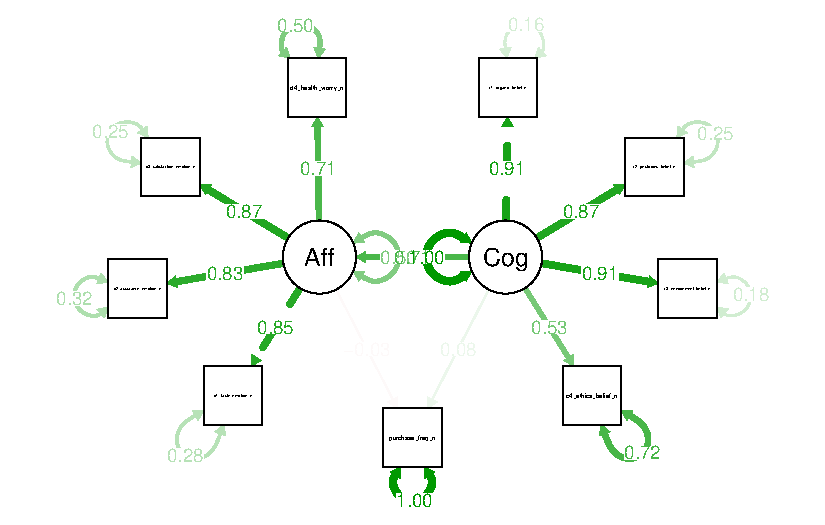
\includegraphics[keepaspectratio]{final_analysis_files/figure-pdf/unnamed-chunk-8-1.pdf}}

\begin{Shaded}
\begin{Highlighting}[]
\CommentTok{\# ── 6.6  Modification indices (for model improvement guidance) ────────────────}

\FunctionTok{cat}\NormalTok{(}\StringTok{"}\SpecialCharTok{\textbackslash{}n}\StringTok{{-}{-}{-} Ha1: Top 10 modification indices {-}{-}{-}}\SpecialCharTok{\textbackslash{}n}\StringTok{"}\NormalTok{)}
\end{Highlighting}
\end{Shaded}

\begin{verbatim}

--- Ha1: Top 10 modification indices ---
\end{verbatim}

\begin{Shaded}
\begin{Highlighting}[]
\FunctionTok{modificationIndices}\NormalTok{(ha1\_fit, }\AttributeTok{sort. =} \ConstantTok{TRUE}\NormalTok{, }\AttributeTok{maximum.number =} \DecValTok{10}\NormalTok{) }\SpecialCharTok{|\textgreater{}} 
  \FunctionTok{print}\NormalTok{()}
\end{Highlighting}
\end{Shaded}

\begin{verbatim}
                       lhs op                       rhs     mi    epc sepc.lv
68       d4_health_worry_n ~~           purchase_freq_n 12.262 -0.287  -0.287
58      c4_ethics_belief_n ~~           purchase_freq_n 11.383 -0.380  -0.380
55      c4_ethics_belief_n ~~    d2_assurance_emotion_n  7.790 -0.162  -0.162
48 c3_environment_belief_n ~~        c4_ethics_belief_n  7.457  0.153   0.153
32                     Aff =~        c4_ethics_belief_n  6.067 -0.371  -0.358
33     c1_organic_belief_n ~~    c2_pesticides_belief_n  5.642  0.117   0.117
41  c2_pesticides_belief_n ~~   c3_environment_belief_n  5.127 -0.111  -0.111
46  c2_pesticides_belief_n ~~         d4_health_worry_n  4.539  0.089   0.089
27                     Cog =~ d3_satisfaction_emotion_n  4.413  0.166   0.176
59      d1_taste_emotion_n ~~    d2_assurance_emotion_n  4.185  0.093   0.093
   sepc.all sepc.nox
68   -0.282   -0.282
58   -0.260   -0.260
55   -0.240   -0.240
48    0.265    0.265
32   -0.261   -0.261
33    0.436    0.436
41   -0.388   -0.388
46    0.191    0.191
27    0.169    0.169
59    0.263    0.263
\end{verbatim}

\begin{Shaded}
\begin{Highlighting}[]
\CommentTok{\# ── 6.7  Plot ─────────────────────────────────────────────────────────────────}

\FunctionTok{ggplot}\NormalTok{(ha1\_data, }\FunctionTok{aes}\NormalTok{(}\AttributeTok{x =}\NormalTok{ Cognitive, }\AttributeTok{y =}\NormalTok{ purchase\_freq\_n)) }\SpecialCharTok{+}
  \FunctionTok{geom\_jitter}\NormalTok{(}\FunctionTok{aes}\NormalTok{(}\AttributeTok{colour =}\NormalTok{ Affective), }\AttributeTok{alpha =} \FloatTok{0.55}\NormalTok{, }\AttributeTok{width =} \FloatTok{0.04}\NormalTok{, }\AttributeTok{height =} \FloatTok{0.15}\NormalTok{) }\SpecialCharTok{+}
  \FunctionTok{geom\_smooth}\NormalTok{(}\AttributeTok{method =} \StringTok{"lm"}\NormalTok{, }\AttributeTok{se =} \ConstantTok{TRUE}\NormalTok{, }\AttributeTok{colour =} \StringTok{"\#2171b5"}\NormalTok{, }\AttributeTok{linewidth =} \DecValTok{1}\NormalTok{) }\SpecialCharTok{+}
  \FunctionTok{scale\_colour\_gradient}\NormalTok{(}\AttributeTok{low =} \StringTok{"\#deebf7"}\NormalTok{, }\AttributeTok{high =} \StringTok{"\#08306b"}\NormalTok{, }\AttributeTok{name =} \StringTok{"Affective}\SpecialCharTok{\textbackslash{}n}\StringTok{Score"}\NormalTok{) }\SpecialCharTok{+}
  \FunctionTok{facet\_wrap}\NormalTok{(}\SpecialCharTok{\textasciitilde{}}\NormalTok{country) }\SpecialCharTok{+}
  \FunctionTok{labs}\NormalTok{(}
    \AttributeTok{title    =} \StringTok{"Ha1: Cognitive Beliefs → Purchase Frequency"}\NormalTok{,}
    \AttributeTok{subtitle =} \StringTok{"Point shade = Affective Emotion composite; line = OLS fit"}\NormalTok{,}
    \AttributeTok{x =} \StringTok{"Cognitive Beliefs (mean score)"}\NormalTok{, }\AttributeTok{y =} \StringTok{"Purchase Frequency (1–6)"}
\NormalTok{  ) }\SpecialCharTok{+}
  \FunctionTok{theme\_study}\NormalTok{()}
\end{Highlighting}
\end{Shaded}

\begin{verbatim}
`geom_smooth()` using formula = 'y ~ x'
\end{verbatim}

\pandocbounded{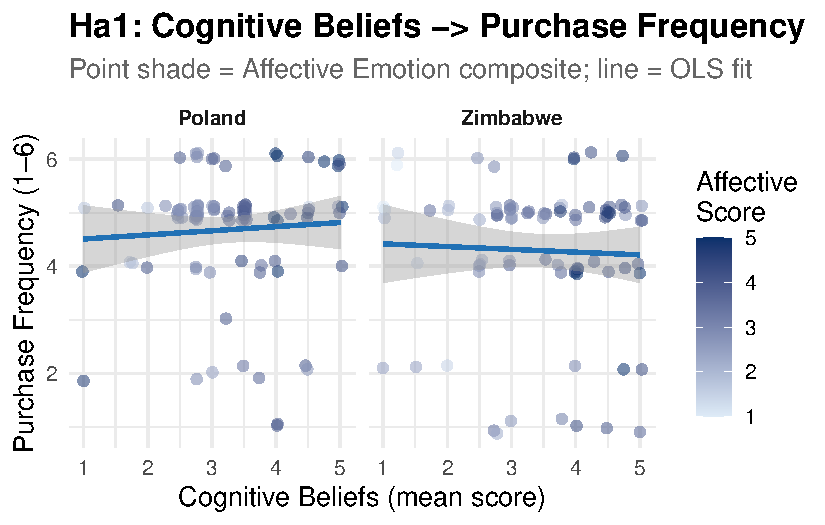
\includegraphics[keepaspectratio]{final_analysis_files/figure-pdf/unnamed-chunk-8-2.pdf}}

\begin{Shaded}
\begin{Highlighting}[]
\CommentTok{\# ggsave("Ha1\_cognitive\_affective\_mediation.png", p\_ha1,}
\CommentTok{\#        width = 10, height = 5, dpi = 300)}
\end{Highlighting}
\end{Shaded}

\subsection{The Theory of the Certification Trust
Chain}\label{the-theory-of-the-certification-trust-chain}

\texttt{Alternative\ (}H₁\texttt{)}: Purchase likelihood is increased by
certification familiarity, which then boosts confidence after the
purchase.

\texttt{Null\ (\textasciigrave{}\textasciigrave{}H₀\textasciigrave{}\textasciigrave{})}:
buy experience does not boost post-buy confidence, and certification
familiarity does not raise purchase likelihood.

\begin{Shaded}
\begin{Highlighting}[]
\CommentTok{\# 7.  Ha2: THEORY OF THE CERTIFICATION TRUST CHAIN}
\CommentTok{\#}
\CommentTok{\#  Path:  Cert Familiarity (C5/C6)}
\CommentTok{\#            → Purchase Frequency (B4)          [a{-}path]}
\CommentTok{\#            → Post{-}purchase Confidence (D2)    [b{-}path]}
\CommentTok{\#  D2 ("I feel confident when I see an organic cert label") is the}
\CommentTok{\#  closest available proxy for post{-}purchase confidence.}


\CommentTok{\# ── 7.1  Complete{-}case dataset for Ha2 ────────────────────────────────────────}

\NormalTok{ha2\_data }\OtherTok{\textless{}{-}}\NormalTok{ df }\SpecialCharTok{|\textgreater{}}
  \FunctionTok{select}\NormalTok{(country, cert\_eu\_n, cert\_zw\_n, cert\_familiar\_n,}
\NormalTok{         cert\_imp\_n, d2\_assurance\_emotion\_n, purchase\_freq\_n, f1\_intent\_n) }\SpecialCharTok{|\textgreater{}}
  \FunctionTok{drop\_na}\NormalTok{()}

\FunctionTok{cat}\NormalTok{(}\FunctionTok{sprintf}\NormalTok{(}\StringTok{"}\SpecialCharTok{\textbackslash{}n}\StringTok{Ha2 n = \%d}\SpecialCharTok{\textbackslash{}n}\StringTok{"}\NormalTok{, }\FunctionTok{nrow}\NormalTok{(ha2\_data)))}
\end{Highlighting}
\end{Shaded}

\begin{verbatim}

Ha2 n = 123
\end{verbatim}

\begin{Shaded}
\begin{Highlighting}[]
\CommentTok{\# ── 7.2  Baron{-}Kenny steps ────────────────────────────────────────────────────}

\CommentTok{\# Step 1: total effect — Cert familiarity → Post{-}purchase confidence (D2)}

\NormalTok{bk1\_ha2 }\OtherTok{\textless{}{-}} \FunctionTok{lm}\NormalTok{(d2\_assurance\_emotion\_n }\SpecialCharTok{\textasciitilde{}}\NormalTok{ cert\_eu\_n }\SpecialCharTok{+}\NormalTok{ cert\_zw\_n, }\AttributeTok{data =}\NormalTok{ ha2\_data)}
\FunctionTok{rob\_test}\NormalTok{(bk1\_ha2, }\StringTok{"Step 1 – Total: Cert familiarity → D2 confidence"}\NormalTok{)}
\end{Highlighting}
\end{Shaded}

\begin{verbatim}

--- Step 1 – Total: Cert familiarity → D2 confidence ---

t test of coefficients:

            Estimate Std. Error t value Pr(>|t|)    
(Intercept) 2.877665   0.270398 10.6423   <2e-16 ***
cert_eu_n   0.182629   0.159092  1.1479   0.2533    
cert_zw_n   0.076818   0.156765  0.4900   0.6250    
---
Signif. codes:  0 '***' 0.001 '**' 0.01 '*' 0.05 '.' 0.1 ' ' 1
\end{verbatim}

\begin{Shaded}
\begin{Highlighting}[]
\CommentTok{\# Step 2: a{-}path — Cert familiarity → Purchase frequency}

\NormalTok{bk2\_ha2 }\OtherTok{\textless{}{-}} \FunctionTok{lm}\NormalTok{(purchase\_freq\_n }\SpecialCharTok{\textasciitilde{}}\NormalTok{ cert\_eu\_n }\SpecialCharTok{+}\NormalTok{ cert\_zw\_n, }\AttributeTok{data =}\NormalTok{ ha2\_data)}
\FunctionTok{rob\_test}\NormalTok{(bk2\_ha2, }\StringTok{"Step 2 – a{-}path: Cert familiarity → Purchase\_Freq"}\NormalTok{)}
\end{Highlighting}
\end{Shaded}

\begin{verbatim}

--- Step 2 – a-path: Cert familiarity → Purchase_Freq ---

t test of coefficients:

            Estimate Std. Error t value  Pr(>|t|)    
(Intercept) 3.683186   0.410964  8.9623 5.032e-15 ***
cert_eu_n   0.092541   0.255600  0.3621    0.7179    
cert_zw_n   0.305020   0.233583  1.3058    0.1941    
---
Signif. codes:  0 '***' 0.001 '**' 0.01 '*' 0.05 '.' 0.1 ' ' 1
\end{verbatim}

\begin{Shaded}
\begin{Highlighting}[]
\CommentTok{\# Step 3: b \& c\textquotesingle{} paths — Cert + Purchase → D2}

\NormalTok{bk3\_ha2 }\OtherTok{\textless{}{-}} \FunctionTok{lm}\NormalTok{(d2\_assurance\_emotion\_n }\SpecialCharTok{\textasciitilde{}}\NormalTok{ cert\_eu\_n }\SpecialCharTok{+}\NormalTok{ cert\_zw\_n }\SpecialCharTok{+}\NormalTok{ purchase\_freq\_n,}
               \AttributeTok{data =}\NormalTok{ ha2\_data)}

\FunctionTok{rob\_test}\NormalTok{(bk3\_ha2, }\StringTok{"Step 3 – b \& c\textquotesingle{} paths: Cert + Purchase → D2 confidence"}\NormalTok{)}
\end{Highlighting}
\end{Shaded}

\begin{verbatim}

--- Step 3 – b & c' paths: Cert + Purchase → D2 confidence ---

t test of coefficients:

                 Estimate Std. Error t value  Pr(>|t|)    
(Intercept)      2.959146   0.361244  8.1916 3.338e-13 ***
cert_eu_n        0.184677   0.161008  1.1470    0.2537    
cert_zw_n        0.083566   0.161859  0.5163    0.6066    
purchase_freq_n -0.022122   0.081122 -0.2727    0.7856    
---
Signif. codes:  0 '***' 0.001 '**' 0.01 '*' 0.05 '.' 0.1 ' ' 1
\end{verbatim}

\begin{Shaded}
\begin{Highlighting}[]
\CommentTok{\# ── 7.3  Sobel test ───────────────────────────────────────────────────────────}

\CommentTok{\# Using EU logo as primary treatment (ZW logo held in model as covariate)}

\FunctionTok{sobel\_test}\NormalTok{(bk2\_ha2, }\AttributeTok{treat =} \StringTok{"cert\_eu\_n"}\NormalTok{, }\AttributeTok{model\_b =}\NormalTok{ bk3\_ha2, }\AttributeTok{mediator =} \StringTok{"purchase\_freq\_n"}\NormalTok{)}
\end{Highlighting}
\end{Shaded}

\begin{verbatim}

--- Sobel Test ---
  Z = -0.2521  |  p = 0.8009
\end{verbatim}

\begin{Shaded}
\begin{Highlighting}[]
\CommentTok{\# ── 7.4  Bootstrapped mediation ───────────────────────────────────────────────}

\FunctionTok{cat}\NormalTok{(}\StringTok{"}\SpecialCharTok{\textbackslash{}n}\StringTok{{-}{-}{-} Ha2: Bootstrapped ACME / ADE / Total (EU logo → Purchase → Confidence) {-}{-}{-}}\SpecialCharTok{\textbackslash{}n}\StringTok{"}\NormalTok{)}
\end{Highlighting}
\end{Shaded}

\begin{verbatim}

--- Ha2: Bootstrapped ACME / ADE / Total (EU logo → Purchase → Confidence) ---
\end{verbatim}

\begin{Shaded}
\begin{Highlighting}[]
\NormalTok{ha2\_med }\OtherTok{\textless{}{-}} \FunctionTok{run\_mediation}\NormalTok{(bk2\_ha2, bk3\_ha2,}
                          \AttributeTok{treat    =} \StringTok{"cert\_eu\_n"}\NormalTok{,}
                          \AttributeTok{mediator =} \StringTok{"purchase\_freq\_n"}\NormalTok{)}
\end{Highlighting}
\end{Shaded}

\begin{verbatim}
Running nonparametric bootstrap
\end{verbatim}

\begin{verbatim}

Causal Mediation Analysis 

Nonparametric Bootstrap Confidence Intervals with the BCa Method

                 Estimate 95% CI Lower 95% CI Upper p-value
ACME           -0.0020472   -0.0401223    0.0490119   0.986
ADE             0.1846767   -0.1149741    0.5221787   0.241
Total Effect    0.1826295   -0.1116704    0.5271670   0.228
Prop. Mediated -0.0112097   -0.1954039    3.0938622   0.995

Sample Size Used: 123 


Simulations: 2000 
\end{verbatim}

\begin{Shaded}
\begin{Highlighting}[]
\CommentTok{\# ── 7.5  SEM ──────────────────────────────────────────────────────────────────}

\NormalTok{ha2\_sem\_spec }\OtherTok{\textless{}{-}} \StringTok{\textquotesingle{}}
\StringTok{  purchase\_freq\_n         \textasciitilde{} a2 * cert\_eu\_n + a2z * cert\_zw\_n}
\StringTok{  d2\_assurance\_emotion\_n  \textasciitilde{} b2 * purchase\_freq\_n +}
\StringTok{                             c2 * cert\_eu\_n + c2z * cert\_zw\_n}
\StringTok{  indirect2 := a2 * b2}
\StringTok{  total2    := c2 + (a2 * b2)}
\StringTok{\textquotesingle{}}

\NormalTok{ha2\_fit }\OtherTok{\textless{}{-}} \FunctionTok{sem}\NormalTok{(ha2\_sem\_spec, }\AttributeTok{data =}\NormalTok{ ha2\_data,}
               \AttributeTok{estimator =} \StringTok{"ML"}\NormalTok{, }\AttributeTok{se =} \StringTok{"bootstrap"}\NormalTok{, }\AttributeTok{bootstrap =} \DecValTok{2000}\NormalTok{)}

\FunctionTok{sem\_fit\_summary}\NormalTok{(ha2\_fit, }\StringTok{"Ha2 SEM Fit Indices"}\NormalTok{)}
\end{Highlighting}
\end{Shaded}

\begin{verbatim}

--- Ha2 SEM Fit Indices ---
Fit indices:
    cfi     tli   rmsea    srmr     aic     bic 
  1.000   1.000   0.000   0.000 729.175 748.860 
\end{verbatim}

\begin{Shaded}
\begin{Highlighting}[]
\FunctionTok{cat}\NormalTok{(}\StringTok{"}\SpecialCharTok{\textbackslash{}n}\StringTok{{-}{-}{-} Ha2: Path estimates {-}{-}{-}}\SpecialCharTok{\textbackslash{}n}\StringTok{"}\NormalTok{)}
\end{Highlighting}
\end{Shaded}

\begin{verbatim}

--- Ha2: Path estimates ---
\end{verbatim}

\begin{Shaded}
\begin{Highlighting}[]
\FunctionTok{sem\_paths}\NormalTok{(ha2\_fit, }\FunctionTok{c}\NormalTok{(}\StringTok{"a2"}\NormalTok{, }\StringTok{"b2"}\NormalTok{, }\StringTok{"c2"}\NormalTok{, }\StringTok{"indirect2"}\NormalTok{, }\StringTok{"total2"}\NormalTok{))}
\end{Highlighting}
\end{Shaded}

\begin{verbatim}
      label    est    se      z pvalue ci.lower ci.upper std.all
1        a2  0.093 0.237  0.391  0.696   -0.360    0.580   0.066
2        b2 -0.022 0.078 -0.285  0.776   -0.181    0.130  -0.027
3        c2  0.185 0.162  1.142  0.253   -0.133    0.499   0.160
4 indirect2 -0.002 0.020 -0.102  0.919   -0.068    0.022  -0.002
5    total2  0.183 0.161  1.135  0.256   -0.139    0.497   0.158
\end{verbatim}

\begin{Shaded}
\begin{Highlighting}[]
\FunctionTok{decide\_indirect}\NormalTok{(ha2\_fit, }\StringTok{"indirect2"}\NormalTok{)}
\end{Highlighting}
\end{Shaded}

\begin{verbatim}

>>> Decision (indirect2): est = -0.002 [-0.068, 0.022]  p = 0.9190
    FAIL TO REJECT H₀ — CI includes zero.
\end{verbatim}

\begin{Shaded}
\begin{Highlighting}[]
\CommentTok{\# ── 7.6  Plot ─────────────────────────────────────────────────────────────────}

\NormalTok{ha2\_data }\SpecialCharTok{|\textgreater{}}
  \FunctionTok{mutate}\NormalTok{(}\AttributeTok{cert\_label =} \FunctionTok{factor}\NormalTok{(cert\_familiar\_n,}
                             \AttributeTok{levels =} \DecValTok{1}\SpecialCharTok{:}\DecValTok{3}\NormalTok{,}
                             \AttributeTok{labels =} \FunctionTok{c}\NormalTok{(}\StringTok{"Unrecognised"}\NormalTok{, }\StringTok{"Seen"}\NormalTok{, }\StringTok{"Familiar"}\NormalTok{))) }\SpecialCharTok{|\textgreater{}}

  \FunctionTok{ggplot}\NormalTok{(}\FunctionTok{aes}\NormalTok{(}\AttributeTok{x =}\NormalTok{ cert\_label, }\AttributeTok{y =}\NormalTok{ d2\_assurance\_emotion\_n)) }\SpecialCharTok{+}
  \FunctionTok{geom\_boxplot}\NormalTok{(}\FunctionTok{aes}\NormalTok{(}\AttributeTok{fill =}\NormalTok{ cert\_label), }\AttributeTok{alpha =} \FloatTok{0.7}\NormalTok{, }\AttributeTok{show.legend =} \ConstantTok{FALSE}\NormalTok{) }\SpecialCharTok{+}
  \FunctionTok{scale\_fill\_brewer}\NormalTok{(}\AttributeTok{palette =} \StringTok{"Greens"}\NormalTok{) }\SpecialCharTok{+}
  \FunctionTok{facet\_wrap}\NormalTok{(}\SpecialCharTok{\textasciitilde{}}\NormalTok{country) }\SpecialCharTok{+}
  \FunctionTok{labs}\NormalTok{(}
    \AttributeTok{title    =} \StringTok{"Ha2: Certification Familiarity → Post{-}purchase Confidence (D2)"}\NormalTok{,}
    \AttributeTok{subtitle =} \StringTok{"Country{-}appropriate logo (EU for Poland; ZW for Zimbabwe)"}\NormalTok{,}
    \AttributeTok{x =} \StringTok{"Certification Familiarity"}\NormalTok{, }\AttributeTok{y =} \StringTok{"D2 Confidence Score (1–5)"}
\NormalTok{  ) }\SpecialCharTok{+}
  \FunctionTok{theme\_study}\NormalTok{()}
\end{Highlighting}
\end{Shaded}

\begin{center}
\pandocbounded{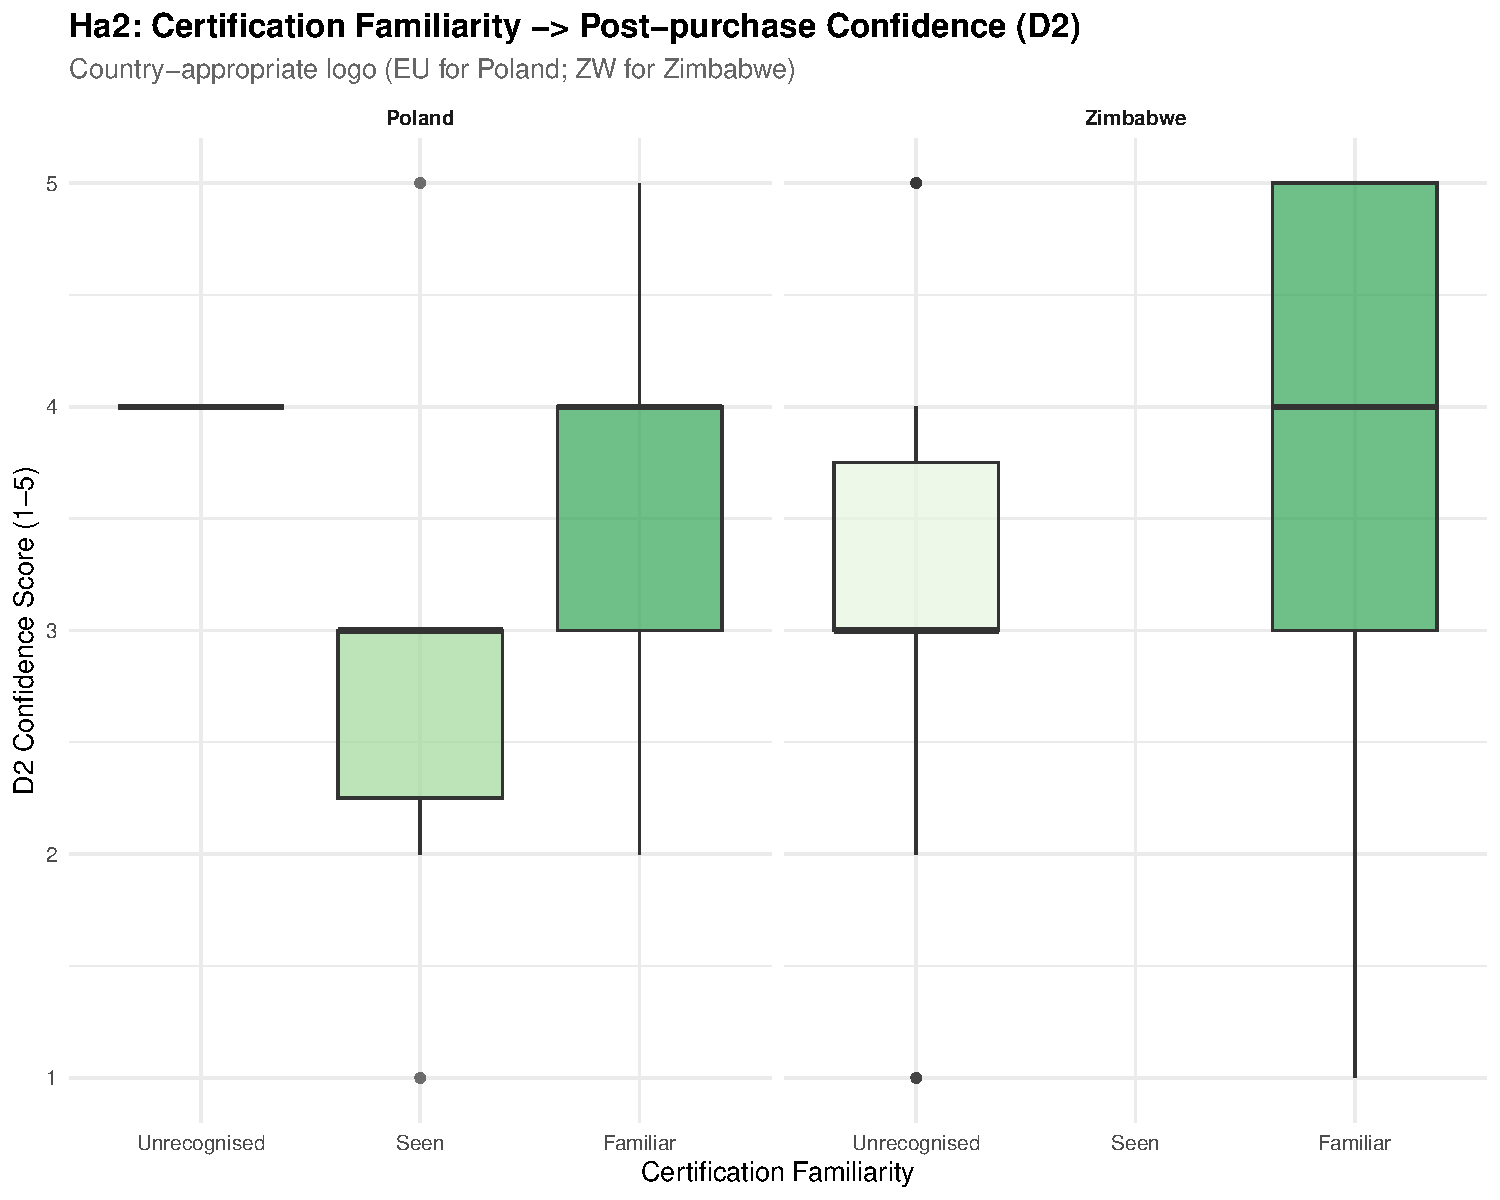
\includegraphics[keepaspectratio]{final_analysis_files/figure-pdf/unnamed-chunk-9-1.pdf}}
\end{center}

\begin{Shaded}
\begin{Highlighting}[]
\CommentTok{\# ggsave("Ha2\_cert\_trust\_chain.png", p\_ha2, width = 10, height = 5, dpi = 300)}
\end{Highlighting}
\end{Shaded}

\subsection{The Moderating Hypothesis of Price
Barriers}\label{the-moderating-hypothesis-of-price-barriers}

\texttt{Alternative\ (H₁)}: The positive correlation between affective
sentiments and purchase intentions is weakened by price perception,
particularly for consumers with lower incomes.

\texttt{Null\ (H₀)}: Regardless of economic level, the link between
affective emotions and purchase intentions is not weakened by price
perception.

\begin{Shaded}
\begin{Highlighting}[]
\CommentTok{\# 8.  Ha3: MODERATING HYPOTHESIS OF PRICE BARRIERS}

\CommentTok{\#  Model:  F1\_intent \textasciitilde{} Affective × Price\_Perception × Employment\_Group}
\CommentTok{\#  Ha3 tests whether high price perception weakens the positive}
\CommentTok{\#  Affective → Intent link, especially among lower{-}SES consumers.}
\CommentTok{\#  Mean{-}centred predictors reduce multicollinearity in interaction terms.}
\CommentTok{\# }
\NormalTok{ha3\_data }\OtherTok{\textless{}{-}}\NormalTok{ df }\SpecialCharTok{|\textgreater{}} 
  \FunctionTok{select}\NormalTok{(country, Affective, Affective\_c, price\_perception\_n, price\_c,}
\NormalTok{         employment\_n, f1\_intent\_n) }\SpecialCharTok{|\textgreater{}}
  \FunctionTok{drop\_na}\NormalTok{()}

\FunctionTok{cat}\NormalTok{(}\FunctionTok{sprintf}\NormalTok{(}\StringTok{"}\SpecialCharTok{\textbackslash{}n}\StringTok{Ha3 n = \%d}\SpecialCharTok{\textbackslash{}n}\StringTok{"}\NormalTok{, }\FunctionTok{nrow}\NormalTok{(ha3\_data)))}
\end{Highlighting}
\end{Shaded}

\begin{verbatim}

Ha3 n = 189
\end{verbatim}

\begin{Shaded}
\begin{Highlighting}[]
\CommentTok{\# ── 8.2  Base 2{-}way moderation: Affective × Price → Intent ───────────────────}

\NormalTok{ha3\_base }\OtherTok{\textless{}{-}} \FunctionTok{lm}\NormalTok{(f1\_intent\_n }\SpecialCharTok{\textasciitilde{}}\NormalTok{ Affective\_c }\SpecialCharTok{*}\NormalTok{ price\_c, }\AttributeTok{data =}\NormalTok{ ha3\_data)}
\FunctionTok{rob\_test}\NormalTok{(ha3\_base, }\StringTok{"Ha3 Base: Affective × Price → F1\_intent"}\NormalTok{)}
\end{Highlighting}
\end{Shaded}

\begin{verbatim}

--- Ha3 Base: Affective × Price → F1_intent ---

t test of coefficients:

                     Estimate Std. Error t value Pr(>|t|)    
(Intercept)          4.429649   0.052879 83.7699   <2e-16 ***
Affective_c          0.081326   0.066773  1.2179   0.2248    
price_c             -0.043564   0.052150 -0.8354   0.4046    
Affective_c:price_c -0.066206   0.065819 -1.0059   0.3158    
---
Signif. codes:  0 '***' 0.001 '**' 0.01 '*' 0.05 '.' 0.1 ' ' 1
\end{verbatim}

\begin{Shaded}
\begin{Highlighting}[]
\FunctionTok{cat}\NormalTok{(}\FunctionTok{sprintf}\NormalTok{(}\StringTok{"  R² = \%.4f}\SpecialCharTok{\textbackslash{}n}\StringTok{"}\NormalTok{, }\FunctionTok{summary}\NormalTok{(ha3\_base)}\SpecialCharTok{$}\NormalTok{r.squared))}
\end{Highlighting}
\end{Shaded}

\begin{verbatim}
  R² = 0.0236
\end{verbatim}

\begin{Shaded}
\begin{Highlighting}[]
\CommentTok{\# ── 8.3  3{-}way moderation: adds Employment as second moderator ────────────────}

\NormalTok{ha3\_3way }\OtherTok{\textless{}{-}} \FunctionTok{lm}\NormalTok{(f1\_intent\_n }\SpecialCharTok{\textasciitilde{}}\NormalTok{ Affective\_c }\SpecialCharTok{*}\NormalTok{ price\_c }\SpecialCharTok{*}\NormalTok{ employment\_n, }\AttributeTok{data =}\NormalTok{ ha3\_data)}
\FunctionTok{rob\_test}\NormalTok{(ha3\_3way, }\StringTok{"Ha3 3{-}Way: Affective × Price × Employment → F1\_intent"}\NormalTok{)}
\end{Highlighting}
\end{Shaded}

\begin{verbatim}

--- Ha3 3-Way: Affective × Price × Employment → F1_intent ---

t test of coefficients:

                                  Estimate Std. Error t value Pr(>|t|)    
(Intercept)                       4.463121   0.223372 19.9806  < 2e-16 ***
Affective_c                      -0.297389   0.256498 -1.1594  0.24781    
price_c                          -0.550919   0.240648 -2.2893  0.02322 *  
employment_n                     -0.015808   0.055318 -0.2858  0.77538    
Affective_c:price_c              -0.455915   0.212691 -2.1436  0.03340 *  
Affective_c:employment_n          0.085037   0.063500  1.3392  0.18219    
price_c:employment_n              0.116124   0.058129  1.9977  0.04725 *  
Affective_c:price_c:employment_n  0.085281   0.055282  1.5427  0.12466    
---
Signif. codes:  0 '***' 0.001 '**' 0.01 '*' 0.05 '.' 0.1 ' ' 1
\end{verbatim}

\begin{Shaded}
\begin{Highlighting}[]
\FunctionTok{cat}\NormalTok{(}\FunctionTok{sprintf}\NormalTok{(}\StringTok{"  R² = \%.4f  |  ΔR² = \%.4f}\SpecialCharTok{\textbackslash{}n}\StringTok{"}\NormalTok{,}
            \FunctionTok{summary}\NormalTok{(ha3\_3way)}\SpecialCharTok{$}\NormalTok{r.squared,}
            \FunctionTok{summary}\NormalTok{(ha3\_3way)}\SpecialCharTok{$}\NormalTok{r.squared }\SpecialCharTok{{-}} \FunctionTok{summary}\NormalTok{(ha3\_base)}\SpecialCharTok{$}\NormalTok{r.squared))}
\end{Highlighting}
\end{Shaded}

\begin{verbatim}
  R² = 0.0654  |  ΔR² = 0.0419
\end{verbatim}

\begin{Shaded}
\begin{Highlighting}[]
\CommentTok{\# ── 8.4  Model comparison via ANOVA ───────────────────────────────────────────}

\FunctionTok{cat}\NormalTok{(}\StringTok{"}\SpecialCharTok{\textbackslash{}n}\StringTok{{-}{-}{-} Ha3: ANOVA — does adding Employment improve fit? {-}{-}{-}}\SpecialCharTok{\textbackslash{}n}\StringTok{"}\NormalTok{)}
\end{Highlighting}
\end{Shaded}

\begin{verbatim}

--- Ha3: ANOVA — does adding Employment improve fit? ---
\end{verbatim}

\begin{Shaded}
\begin{Highlighting}[]
\FunctionTok{print}\NormalTok{(}\FunctionTok{anova}\NormalTok{(ha3\_base, ha3\_3way))}
\end{Highlighting}
\end{Shaded}

\begin{verbatim}
Analysis of Variance Table

Model 1: f1_intent_n ~ Affective_c * price_c
Model 2: f1_intent_n ~ Affective_c * price_c * employment_n
  Res.Df    RSS Df Sum of Sq     F  Pr(>F)  
1    185 95.968                             
2    181 91.854  4    4.1146 2.027 0.09249 .
---
Signif. codes:  0 '***' 0.001 '**' 0.01 '*' 0.05 '.' 0.1 ' ' 1
\end{verbatim}

\begin{Shaded}
\begin{Highlighting}[]
\CommentTok{\# ── 8.5  Simple slopes by employment tier ─────────────────────────────────────}

\CommentTok{\# Low = 1–2 (part{-}time / full{-}time employed at lower scale)}

\CommentTok{\# High = 5–6 (retired / student — proxy for constrained income)}

\CommentTok{\# simple\_slopes \textless{}{-} function(emp\_vals, label) \{}
\CommentTok{\#   m \textless{}{-} lm(f1\_intent\_n \textasciitilde{} Affective\_c * price\_c,}
\CommentTok{\#           data = filter(ha3\_data, employment\_n \%in\% emp\_vals))}
\CommentTok{\#   rob\_test(m, paste("Simple slopes —", label))}
\CommentTok{\# \}}
\CommentTok{\# }
\CommentTok{\# simple\_slopes(1:2, "Lower employment tier")}
\CommentTok{\# simple\_slopes(5:7, "Higher/non{-}employment tier")}

\CommentTok{\# ── 8.6  Johnson{-}Neyman interval ─────────────────────────────────────────────}

\FunctionTok{cat}\NormalTok{(}\StringTok{"}\SpecialCharTok{\textbackslash{}n}\StringTok{{-}{-}{-} Ha3: Johnson{-}Neyman — where is price moderation significant? {-}{-}{-}}\SpecialCharTok{\textbackslash{}n}\StringTok{"}\NormalTok{)}
\end{Highlighting}
\end{Shaded}

\begin{verbatim}

--- Ha3: Johnson-Neyman — where is price moderation significant? ---
\end{verbatim}

\begin{Shaded}
\begin{Highlighting}[]
\NormalTok{jn }\OtherTok{\textless{}{-}}\NormalTok{ interactions}\SpecialCharTok{::}\FunctionTok{johnson\_neyman}\NormalTok{(}
  \AttributeTok{model =}\NormalTok{ ha3\_base, }\AttributeTok{pred =} \StringTok{"Affective\_c"}\NormalTok{, }\AttributeTok{modx =} \StringTok{"price\_c"}\NormalTok{, }\AttributeTok{alpha =} \FloatTok{0.05}
\NormalTok{)}

\FunctionTok{print}\NormalTok{(jn)}
\end{Highlighting}
\end{Shaded}

\begin{verbatim}
JOHNSON-NEYMAN INTERVAL

The Johnson-Neyman interval could not be found. Is the p value for your
interaction term below the specified alpha?
\end{verbatim}

\begin{center}
\pandocbounded{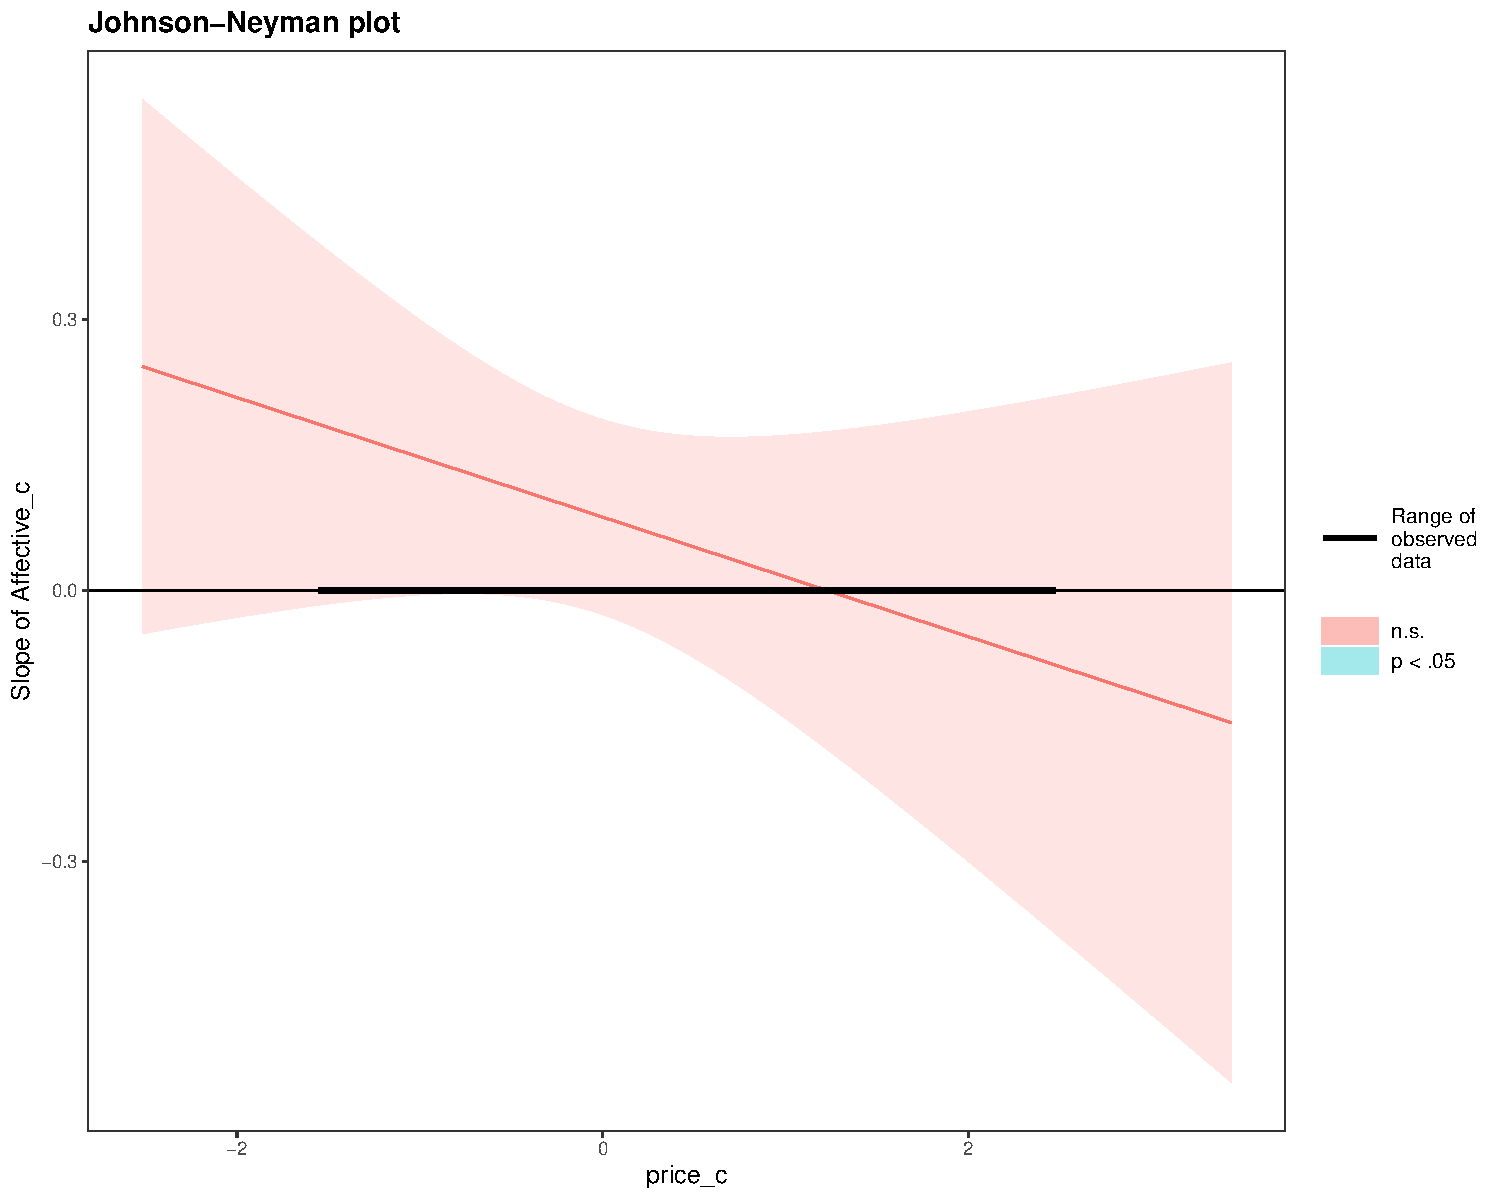
\includegraphics[keepaspectratio]{final_analysis_files/figure-pdf/unnamed-chunk-10-1.pdf}}
\end{center}

\begin{Shaded}
\begin{Highlighting}[]
\CommentTok{\# ── 8.8  Plot ─────────────────────────────────────────────────────────────────}

\CommentTok{\# interactions::interact\_plot(}
\CommentTok{\#   ha3\_3way,}
\CommentTok{\#   pred        = Affective,}
\CommentTok{\#   modx        = price\_perception\_num,}
\CommentTok{\#   mod2        = employment\_n,}
\CommentTok{\#   modx.values = c({-}1, 0, 1),}
\CommentTok{\#   x.label     = "Affective Emotions (mean{-}centred)",}
\CommentTok{\#   y.label     = "Purchase Intention (F1)",}
\CommentTok{\#   legend.main = "Price Barrier\textbackslash{}n(±1 SD)",}
\CommentTok{\#   main.title  = "Ha3: Affective × Price × Employment → Purchase Intention") +}
\CommentTok{\#   theme\_study()}


\CommentTok{\# ggsave("Ha3\_price\_moderation.png", p\_ha3, width = 11, height = 6, dpi = 300)}
\end{Highlighting}
\end{Shaded}

\subsection{\texorpdfstring{\textbf{Hypothesis of Country-Specific
Demographic
Drivers}}{Hypothesis of Country-Specific Demographic Drivers}}\label{hypothesis-of-country-specific-demographic-drivers}

\texttt{Alternative\ (H₁)}: In both nations, socioeconomic position has
a favorable impact on cognitive beliefs and purchase frequency, but it
does so through distinct mechanisms---directly in Zimbabwe and
indirectly through education and urban residency in Poland.

\texttt{Null\ (H₀)}: Neither country's cognitive views nor purchase
frequency are significantly impacted by socioeconomic position.

\begin{Shaded}
\begin{Highlighting}[]
\CommentTok{\# 9.  Ha4: COUNTRY{-}SPECIFIC DEMOGRAPHIC DRIVERS}
\CommentTok{\#}
\CommentTok{\#  Hypothesis:}
\CommentTok{\#    Zimbabwe — SES affects Cognitive Beliefs and Purchase Frequency DIRECTLY}
\CommentTok{\#    Poland   — SES operates INDIRECTLY via Education \& Urban residency → Cognitive}
\CommentTok{\#}
\CommentTok{\#  SEP composite = mean(household\_econ\_n, education\_n, employment\_n)}


\CommentTok{\# ── 9.1  Country subsets ──────────────────────────────────────────────────────}

\NormalTok{ha4\_data }\OtherTok{\textless{}{-}}\NormalTok{ df }\SpecialCharTok{|\textgreater{}}
  \FunctionTok{select}\NormalTok{(country, SEP, household\_econ\_n, education\_n, employment\_n,}
\NormalTok{         Cognitive, purchase\_freq\_n) }\SpecialCharTok{|\textgreater{}}
   \FunctionTok{drop\_na}\NormalTok{()}


\NormalTok{df\_pol }\OtherTok{\textless{}{-}} \FunctionTok{filter}\NormalTok{(ha4\_data, country }\SpecialCharTok{==} \StringTok{"Poland"}\NormalTok{)}

\NormalTok{df\_zim }\OtherTok{\textless{}{-}} \FunctionTok{filter}\NormalTok{(ha4\_data, country }\SpecialCharTok{==} \StringTok{"Zimbabwe"}\NormalTok{)}

\FunctionTok{cat}\NormalTok{(}\FunctionTok{sprintf}\NormalTok{(}\StringTok{"}\SpecialCharTok{\textbackslash{}n}\StringTok{Ha4: n(Poland) = \%d  |  n(Zimbabwe) = \%d}\SpecialCharTok{\textbackslash{}n}\StringTok{"}\NormalTok{,}
            \FunctionTok{nrow}\NormalTok{(df\_pol), }\FunctionTok{nrow}\NormalTok{(df\_zim)))}
\end{Highlighting}
\end{Shaded}

\begin{verbatim}

Ha4: n(Poland) = 90  |  n(Zimbabwe) = 82
\end{verbatim}

\begin{Shaded}
\begin{Highlighting}[]
\CommentTok{\# ── 9.2  OLS by country (baseline robustness check) ──────────────────────────}

\NormalTok{ols\_pol }\OtherTok{\textless{}{-}} \FunctionTok{lm}\NormalTok{(purchase\_freq\_n }\SpecialCharTok{\textasciitilde{}}\NormalTok{ SEP }\SpecialCharTok{+}\NormalTok{ education\_n }\SpecialCharTok{+}\NormalTok{ Cognitive, }\AttributeTok{data =}\NormalTok{ df\_pol)}

\NormalTok{ols\_zim }\OtherTok{\textless{}{-}} \FunctionTok{lm}\NormalTok{(purchase\_freq\_n }\SpecialCharTok{\textasciitilde{}}\NormalTok{ SEP }\SpecialCharTok{+}\NormalTok{ education\_n }\SpecialCharTok{+}\NormalTok{ Cognitive, }\AttributeTok{data =}\NormalTok{ df\_zim)}

\FunctionTok{rob\_test}\NormalTok{(ols\_pol, }
         \StringTok{"Ha4 OLS — Poland: SEP + Education + Cognitive → Purchase\_Freq"}\NormalTok{)}
\end{Highlighting}
\end{Shaded}

\begin{verbatim}

--- Ha4 OLS — Poland: SEP + Education + Cognitive → Purchase_Freq ---

t test of coefficients:

             Estimate Std. Error t value Pr(>|t|)   
(Intercept)  2.881287   1.030488  2.7960  0.00638 **
SEP          0.563432   0.283226  1.9893  0.04984 * 
education_n -0.105529   0.177436 -0.5947  0.55358   
Cognitive    0.052528   0.131530  0.3994  0.69062   
---
Signif. codes:  0 '***' 0.001 '**' 0.01 '*' 0.05 '.' 0.1 ' ' 1
\end{verbatim}

\begin{Shaded}
\begin{Highlighting}[]
\FunctionTok{rob\_test}\NormalTok{(ols\_zim, }
         \StringTok{"Ha4 OLS — Zimbabwe: SEP + Education + Cognitive → Purchase\_Freq"}\NormalTok{)}
\end{Highlighting}
\end{Shaded}

\begin{verbatim}

--- Ha4 OLS — Zimbabwe: SEP + Education + Cognitive → Purchase_Freq ---

t test of coefficients:

             Estimate Std. Error t value  Pr(>|t|)    
(Intercept)  4.547940   1.034165  4.3977 3.421e-05 ***
SEP         -0.053920   0.381699 -0.1413    0.8880    
education_n  0.032054   0.328921  0.0975    0.9226    
Cognitive   -0.052874   0.156825 -0.3372    0.7369    
---
Signif. codes:  0 '***' 0.001 '**' 0.01 '*' 0.05 '.' 0.1 ' ' 1
\end{verbatim}

\begin{Shaded}
\begin{Highlighting}[]
\CommentTok{\# ── 9.3  Chow structural{-}break test ──────────────────────────────────────────}

\NormalTok{ols\_pool }\OtherTok{\textless{}{-}} \FunctionTok{lm}\NormalTok{(purchase\_freq\_n }\SpecialCharTok{\textasciitilde{}}\NormalTok{ SEP }\SpecialCharTok{+}\NormalTok{ education\_n }\SpecialCharTok{+}\NormalTok{ Cognitive, }\AttributeTok{data =}\NormalTok{ ha4\_data)}

\NormalTok{rss\_pool }\OtherTok{\textless{}{-}} \FunctionTok{sum}\NormalTok{(}\FunctionTok{resid}\NormalTok{(ols\_pool)}\SpecialCharTok{\^{}}\DecValTok{2}\NormalTok{)}
\NormalTok{rss\_split }\OtherTok{\textless{}{-}} \FunctionTok{sum}\NormalTok{(}\FunctionTok{resid}\NormalTok{(ols\_pol)}\SpecialCharTok{\^{}}\DecValTok{2}\NormalTok{) }\SpecialCharTok{+} \FunctionTok{sum}\NormalTok{(}\FunctionTok{resid}\NormalTok{(ols\_zim)}\SpecialCharTok{\^{}}\DecValTok{2}\NormalTok{)}
\NormalTok{k  }\OtherTok{\textless{}{-}} \FunctionTok{length}\NormalTok{(}\FunctionTok{coef}\NormalTok{(ols\_pool))}
\NormalTok{n\_total    }\OtherTok{\textless{}{-}} \FunctionTok{nrow}\NormalTok{(ha4\_data)}
\NormalTok{chow\_F     }\OtherTok{\textless{}{-}}\NormalTok{ ((rss\_pool }\SpecialCharTok{{-}}\NormalTok{ rss\_split) }\SpecialCharTok{/}\NormalTok{ k) }\SpecialCharTok{/}\NormalTok{ (rss\_split }\SpecialCharTok{/}\NormalTok{ (n\_total }\SpecialCharTok{{-}} \DecValTok{2} \SpecialCharTok{*}\NormalTok{ k))}
\NormalTok{chow\_p     }\OtherTok{\textless{}{-}} \FunctionTok{pf}\NormalTok{(chow\_F, }\AttributeTok{df1 =}\NormalTok{ k, }\AttributeTok{df2 =}\NormalTok{ n\_total }\SpecialCharTok{{-}} \DecValTok{2} \SpecialCharTok{*}\NormalTok{ k, }\AttributeTok{lower.tail =} \ConstantTok{FALSE}\NormalTok{)}

\FunctionTok{cat}\NormalTok{(}\FunctionTok{sprintf}\NormalTok{(}\StringTok{"}\SpecialCharTok{\textbackslash{}n}\StringTok{{-}{-}{-} Chow Test: F(\%d, \%d) = \%.4f  p = \%.6f {-}{-}{-}}\SpecialCharTok{\textbackslash{}n}\StringTok{"}\NormalTok{,}
\NormalTok{            k, n\_total }\SpecialCharTok{{-}} \DecValTok{2} \SpecialCharTok{*}\NormalTok{ k, chow\_F, chow\_p))}
\end{Highlighting}
\end{Shaded}

\begin{verbatim}

--- Chow Test: F(4, 164) = 1.5537  p = 0.189154 ---
\end{verbatim}

\begin{Shaded}
\begin{Highlighting}[]
\CommentTok{\# ── 9.4  Multi{-}group SEM (free vs constrained) ────────────────────────────────}

\CommentTok{\# The model encodes both country pathways simultaneously.}

\CommentTok{\# Poland pathway: SEP → Education → Cognitive → Purchase (indirect)}

\CommentTok{\# Zimbabwe pathway: SEP → Cognitive \& Purchase directly}

\NormalTok{ha4\_sem\_spec }\OtherTok{\textless{}{-}} \StringTok{\textquotesingle{}}
\StringTok{  \# Poland mechanism: SEP flows through education to cognitive beliefs}
\StringTok{  education\_n    \textasciitilde{} m\_edu * SEP}
\StringTok{  \# Cognitive beliefs: driven by SEP and (for Poland) education}
\StringTok{  Cognitive      \textasciitilde{} a\_sep * SEP + a\_edu * education\_n}
\StringTok{  \# Purchase frequency: direct SEP effect + through cognition}
\StringTok{  purchase\_freq\_n \textasciitilde{} b\_cog * Cognitive + d\_sep * SEP}
\StringTok{  \# Defined indirect effects}
\StringTok{  indirect\_sep\_cog  := a\_sep * b\_cog}
\StringTok{  indirect\_edu\_path := m\_edu * a\_edu * b\_cog}
\StringTok{  total\_indirect    := indirect\_sep\_cog + indirect\_edu\_path}
\StringTok{  total\_sep\_effect  := d\_sep + total\_indirect}
\StringTok{\textquotesingle{}}

\CommentTok{\# Free model: all paths estimated separately per country}

\NormalTok{ha4\_free }\OtherTok{\textless{}{-}} \FunctionTok{sem}\NormalTok{(ha4\_sem\_spec, }\AttributeTok{data =}\NormalTok{ ha4\_data, }
                \AttributeTok{group =} \StringTok{"country"}\NormalTok{,}
                \AttributeTok{estimator =} \StringTok{"ML"}\NormalTok{, }
                \AttributeTok{se =} \StringTok{"bootstrap"}\NormalTok{, }\AttributeTok{bootstrap =} \DecValTok{1000}\NormalTok{,}
                \AttributeTok{missing =} \StringTok{"ml"}\NormalTok{)}
\end{Highlighting}
\end{Shaded}

\begin{verbatim}
Warning: lavaan->lavParTable():  
   using a single label per parameter in a multiple group setting implies 
   imposing equality constraints across all the groups; If this is not 
   intended, either remove the label(s), or use a vector of labels (one for 
   each group); See the Multiple groups section in the man page of 
   model.syntax.
\end{verbatim}

\begin{Shaded}
\begin{Highlighting}[]
\CommentTok{\# Constrained model: regression paths forced equal across countries (null model)}

\NormalTok{ha4\_const }\OtherTok{\textless{}{-}} \FunctionTok{sem}\NormalTok{(ha4\_sem\_spec, }\AttributeTok{data =}\NormalTok{ ha4\_data, }\AttributeTok{group =} \StringTok{"country"}\NormalTok{,}
                 \AttributeTok{group.equal =} \StringTok{"regressions"}\NormalTok{,}
                 \AttributeTok{estimator =} \StringTok{"ML"}\NormalTok{, }\AttributeTok{se =} \StringTok{"bootstrap"}\NormalTok{, }\AttributeTok{bootstrap =} \DecValTok{1000}\NormalTok{,}
                 \AttributeTok{missing =} \StringTok{"ml"}\NormalTok{)}

\FunctionTok{sem\_fit\_summary}\NormalTok{(ha4\_free, }\StringTok{"Ha4 Free (unconstrained) Model"}\NormalTok{)}
\end{Highlighting}
\end{Shaded}

\begin{verbatim}

--- Ha4 Free (unconstrained) Model ---
Fit indices:
     cfi      tli    rmsea     srmr      aic      bic 
   0.991    0.984    0.038    0.064 1409.005 1462.512 
\end{verbatim}

\begin{Shaded}
\begin{Highlighting}[]
\FunctionTok{cat}\NormalTok{(}\StringTok{"}\SpecialCharTok{\textbackslash{}n}\StringTok{{-}{-}{-} Ha4: Δχ² test — free vs constrained {-}{-}{-}}\SpecialCharTok{\textbackslash{}n}\StringTok{"}\NormalTok{)}
\end{Highlighting}
\end{Shaded}

\begin{verbatim}

--- Ha4: Δχ² test — free vs constrained ---
\end{verbatim}

\begin{Shaded}
\begin{Highlighting}[]
\FunctionTok{print}\NormalTok{(}\FunctionTok{lavTestLRT}\NormalTok{(ha4\_free, ha4\_const))}
\end{Highlighting}
\end{Shaded}

\begin{verbatim}
Warning: lavaan->lavTestLRT():  
   some models have the same degrees of freedom
\end{verbatim}

\begin{verbatim}

Chi-Squared Difference Test

          Df  AIC    BIC  Chisq Chisq diff Df diff Pr(>Chisq)
ha4_free   7 1409 1462.5 7.8771                              
ha4_const  7 1409 1462.5 7.8771          0       0           
\end{verbatim}

\begin{Shaded}
\begin{Highlighting}[]
\CommentTok{\# Per{-}country structural path estimates}

\NormalTok{pe\_free }\OtherTok{\textless{}{-}} \FunctionTok{parameterEstimates}\NormalTok{(ha4\_free, }\AttributeTok{boot.ci.type =} \StringTok{"bca.simple"}\NormalTok{, }\AttributeTok{ci =} \ConstantTok{TRUE}\NormalTok{) }\SpecialCharTok{|\textgreater{}}
  \FunctionTok{filter}\NormalTok{(op }\SpecialCharTok{\%in\%} \FunctionTok{c}\NormalTok{(}\StringTok{"\textasciitilde{}"}\NormalTok{, }\StringTok{":="}\NormalTok{)) }\SpecialCharTok{|\textgreater{}}
  \FunctionTok{select}\NormalTok{(lhs, op, rhs, group, est, se, pvalue, ci.lower, ci.upper)}

\FunctionTok{cat}\NormalTok{(}\StringTok{"}\SpecialCharTok{\textbackslash{}n}\StringTok{{-}{-}{-} Ha4: Poland paths (group = 1) {-}{-}{-}}\SpecialCharTok{\textbackslash{}n}\StringTok{"}\NormalTok{)}
\end{Highlighting}
\end{Shaded}

\begin{verbatim}

--- Ha4: Poland paths (group = 1) ---
\end{verbatim}

\begin{Shaded}
\begin{Highlighting}[]
\FunctionTok{print}\NormalTok{(}\FunctionTok{filter}\NormalTok{(pe\_free, group }\SpecialCharTok{==} \DecValTok{1}\NormalTok{))}
\end{Highlighting}
\end{Shaded}

\begin{verbatim}
              lhs op         rhs group   est    se pvalue ci.lower ci.upper
1     education_n  ~         SEP     1 0.908 0.076  0.000    0.748    1.048
2       Cognitive  ~         SEP     1 0.015 0.174  0.929   -0.299    0.405
3       Cognitive  ~ education_n     1 0.151 0.130  0.247   -0.104    0.403
4 purchase_freq_n  ~   Cognitive     1 0.000 0.096  1.000   -0.192    0.184
5 purchase_freq_n  ~         SEP     1 0.287 0.192  0.134   -0.125    0.625
\end{verbatim}

\begin{Shaded}
\begin{Highlighting}[]
\FunctionTok{cat}\NormalTok{(}\StringTok{"}\SpecialCharTok{\textbackslash{}n}\StringTok{{-}{-}{-} Ha4: Zimbabwe paths (group = 2) {-}{-}{-}}\SpecialCharTok{\textbackslash{}n}\StringTok{"}\NormalTok{)}
\end{Highlighting}
\end{Shaded}

\begin{verbatim}

--- Ha4: Zimbabwe paths (group = 2) ---
\end{verbatim}

\begin{Shaded}
\begin{Highlighting}[]
\FunctionTok{print}\NormalTok{(}\FunctionTok{filter}\NormalTok{(pe\_free, group }\SpecialCharTok{==} \DecValTok{2}\NormalTok{))}
\end{Highlighting}
\end{Shaded}

\begin{verbatim}
              lhs op         rhs group   est    se pvalue ci.lower ci.upper
1     education_n  ~         SEP     2 0.908 0.076  0.000    0.748    1.048
2       Cognitive  ~         SEP     2 0.015 0.174  0.929   -0.299    0.405
3       Cognitive  ~ education_n     2 0.151 0.130  0.247   -0.104    0.403
4 purchase_freq_n  ~   Cognitive     2 0.000 0.096  1.000   -0.192    0.184
5 purchase_freq_n  ~         SEP     2 0.287 0.192  0.134   -0.125    0.625
\end{verbatim}

\begin{Shaded}
\begin{Highlighting}[]
\CommentTok{\# ── 9.5  Country{-}specific mediation confirmatory tests ────────────────────────}

\CommentTok{\# Poland: SEP → Education (mediator) → Cognitive → Purchase}

\FunctionTok{cat}\NormalTok{(}\StringTok{"}\SpecialCharTok{\textbackslash{}n}\StringTok{{-}{-}{-} Ha4 Poland: SES → Education → Cognitive (mediation) {-}{-}{-}}\SpecialCharTok{\textbackslash{}n}\StringTok{"}\NormalTok{)}
\end{Highlighting}
\end{Shaded}

\begin{verbatim}

--- Ha4 Poland: SES → Education → Cognitive (mediation) ---
\end{verbatim}

\begin{Shaded}
\begin{Highlighting}[]
\NormalTok{pol\_m }\OtherTok{\textless{}{-}} \FunctionTok{lm}\NormalTok{(education\_n }\SpecialCharTok{\textasciitilde{}}\NormalTok{ SEP, }\AttributeTok{data =}\NormalTok{ df\_pol)}
\NormalTok{pol\_y }\OtherTok{\textless{}{-}} \FunctionTok{lm}\NormalTok{(Cognitive }\SpecialCharTok{\textasciitilde{}}\NormalTok{ SEP }\SpecialCharTok{+}\NormalTok{ education\_n, }\AttributeTok{data =}\NormalTok{ df\_pol)}

\NormalTok{ha4\_med\_pol }\OtherTok{\textless{}{-}} \FunctionTok{run\_mediation}\NormalTok{(pol\_m, pol\_y, }\AttributeTok{treat =} \StringTok{"SEP"}\NormalTok{, }\AttributeTok{mediator =} \StringTok{"education\_n"}\NormalTok{,}
                              \AttributeTok{sims =} \DecValTok{1000}\NormalTok{)}
\end{Highlighting}
\end{Shaded}

\begin{verbatim}
Running nonparametric bootstrap
\end{verbatim}

\begin{verbatim}

Causal Mediation Analysis 

Nonparametric Bootstrap Confidence Intervals with the BCa Method

                Estimate 95% CI Lower 95% CI Upper p-value
ACME            0.060229    -0.269756     0.369809   0.742
ADE             0.058371    -0.412672     0.524374   0.820
Total Effect    0.118600    -0.312377     0.477827   0.622
Prop. Mediated  0.507836    -3.121160    32.953989   0.800

Sample Size Used: 90 


Simulations: 1000 
\end{verbatim}

\begin{Shaded}
\begin{Highlighting}[]
\CommentTok{\# Zimbabwe: SEP → Cognitive (mediator) → Purchase}

\FunctionTok{cat}\NormalTok{(}\StringTok{"}\SpecialCharTok{\textbackslash{}n}\StringTok{{-}{-}{-} Ha4 Zimbabwe: SES → Cognitive → Purchase (mediation) {-}{-}{-}}\SpecialCharTok{\textbackslash{}n}\StringTok{"}\NormalTok{)}
\end{Highlighting}
\end{Shaded}

\begin{verbatim}

--- Ha4 Zimbabwe: SES → Cognitive → Purchase (mediation) ---
\end{verbatim}

\begin{Shaded}
\begin{Highlighting}[]
\NormalTok{zim\_m }\OtherTok{\textless{}{-}} \FunctionTok{lm}\NormalTok{(Cognitive  }\SpecialCharTok{\textasciitilde{}}\NormalTok{ SEP, }\AttributeTok{data =}\NormalTok{ df\_zim)}
\NormalTok{zim\_y }\OtherTok{\textless{}{-}} \FunctionTok{lm}\NormalTok{(purchase\_freq\_n }\SpecialCharTok{\textasciitilde{}}\NormalTok{ SEP }\SpecialCharTok{+}\NormalTok{ Cognitive, }\AttributeTok{data =}\NormalTok{ df\_zim)}

\NormalTok{ha4\_med\_zim }\OtherTok{\textless{}{-}} \FunctionTok{run\_mediation}\NormalTok{(zim\_m, zim\_y, }\AttributeTok{treat =} \StringTok{"SEP"}\NormalTok{, }\AttributeTok{mediator =} \StringTok{"Cognitive"}\NormalTok{,}
                              \AttributeTok{sims =} \DecValTok{1000}\NormalTok{)}
\end{Highlighting}
\end{Shaded}

\begin{verbatim}
Running nonparametric bootstrap
\end{verbatim}

\begin{verbatim}

Causal Mediation Analysis 

Nonparametric Bootstrap Confidence Intervals with the BCa Method

                  Estimate 95% CI Lower 95% CI Upper p-value
ACME           -1.1360e-02  -1.8548e-01   4.3549e-02   0.746
ADE            -3.0218e-02  -5.4049e-01   4.5832e-01   0.830
Total Effect   -4.1578e-02  -5.4842e-01   4.6192e-01   0.802
Prop. Mediated  2.7323e-01   9.5178e+13   9.7771e+13   0.908

Sample Size Used: 82 


Simulations: 1000 
\end{verbatim}

\begin{Shaded}
\begin{Highlighting}[]
\CommentTok{\# ── 9.6  Decision ─────────────────────────────────────────────────────────────}

\NormalTok{lrt\_result }\OtherTok{\textless{}{-}} \FunctionTok{lavTestLRT}\NormalTok{(ha4\_free, ha4\_const)}
\end{Highlighting}
\end{Shaded}

\begin{verbatim}
Warning: lavaan->lavTestLRT():  
   some models have the same degrees of freedom
\end{verbatim}

\begin{Shaded}
\begin{Highlighting}[]
\NormalTok{delta\_p    }\OtherTok{\textless{}{-}}\NormalTok{ lrt\_result[[}\StringTok{"Pr(\textgreater{}Chisq)"}\NormalTok{]][}\DecValTok{2}\NormalTok{]}

\FunctionTok{cat}\NormalTok{(}\StringTok{"}\SpecialCharTok{\textbackslash{}n}\StringTok{\textgreater{}\textgreater{}\textgreater{} Ha4 Decision:}\SpecialCharTok{\textbackslash{}n}\StringTok{"}\NormalTok{)}
\end{Highlighting}
\end{Shaded}

\begin{verbatim}

>>> Ha4 Decision:
\end{verbatim}

\begin{Shaded}
\begin{Highlighting}[]
\FunctionTok{cat}\NormalTok{(}\FunctionTok{sprintf}\NormalTok{(}\StringTok{"  Chow test: F = \%.4f  p = \%.4f  →  \%s}\SpecialCharTok{\textbackslash{}n}\StringTok{"}\NormalTok{,}
\NormalTok{            chow\_F, chow\_p,}
            \ControlFlowTok{if}\NormalTok{ (chow\_p }\SpecialCharTok{\textless{}} \FloatTok{0.05}\NormalTok{) }\StringTok{"REJECT H\textbackslash{}u2080 (structural break confirmed)"}
            \ControlFlowTok{else} \StringTok{"FAIL TO REJECT H\textbackslash{}u2080"}\NormalTok{))}
\end{Highlighting}
\end{Shaded}

\begin{verbatim}
  Chow test: F = 1.5537  p = 0.1892  →  FAIL TO REJECT H₀
\end{verbatim}

\begin{Shaded}
\begin{Highlighting}[]
\CommentTok{\# ── 9.7  Coefficient plot (Poland vs Zimbabwe) ────────────────────────────────}

\NormalTok{coef\_tbl }\OtherTok{\textless{}{-}} \FunctionTok{bind\_rows}\NormalTok{(}
  \FunctionTok{tidy}\NormalTok{(ols\_pol, }\AttributeTok{conf.int =} \ConstantTok{TRUE}\NormalTok{) }\SpecialCharTok{|\textgreater{}} \FunctionTok{mutate}\NormalTok{(}\AttributeTok{Country =} \StringTok{"Poland"}\NormalTok{),}
  \FunctionTok{tidy}\NormalTok{(ols\_zim, }\AttributeTok{conf.int =} \ConstantTok{TRUE}\NormalTok{) }\SpecialCharTok{|\textgreater{}} \FunctionTok{mutate}\NormalTok{(}\AttributeTok{Country =} \StringTok{"Zimbabwe"}\NormalTok{)}
\NormalTok{) }\SpecialCharTok{|\textgreater{}}
  \FunctionTok{filter}\NormalTok{(term }\SpecialCharTok{!=} \StringTok{"(Intercept)"}\NormalTok{) }\SpecialCharTok{|\textgreater{}}
  \FunctionTok{mutate}\NormalTok{(}\AttributeTok{term =} \FunctionTok{recode}\NormalTok{(term,}
    \StringTok{"SEP"}         \OtherTok{=} \StringTok{"SEP (composite)"}\NormalTok{,}
    \StringTok{"education\_n"} \OtherTok{=} \StringTok{"Education"}\NormalTok{,}
    \StringTok{"Cognitive"}   \OtherTok{=} \StringTok{"Cognitive Beliefs"}
\NormalTok{  ))}

\FunctionTok{ggplot}\NormalTok{(coef\_tbl,}
                \FunctionTok{aes}\NormalTok{(}\AttributeTok{x =}\NormalTok{ estimate, }\AttributeTok{y =}\NormalTok{ term, }\AttributeTok{colour =}\NormalTok{ Country,}
                    \AttributeTok{xmin =}\NormalTok{ conf.low, }\AttributeTok{xmax =}\NormalTok{ conf.high)) }\SpecialCharTok{+}
  \FunctionTok{geom\_vline}\NormalTok{(}\AttributeTok{xintercept =} \DecValTok{0}\NormalTok{, }\AttributeTok{linetype =} \StringTok{"dashed"}\NormalTok{, }\AttributeTok{colour =} \StringTok{"grey60"}\NormalTok{) }\SpecialCharTok{+}
  \FunctionTok{geom\_pointrange}\NormalTok{(}\AttributeTok{position =} \FunctionTok{position\_dodge}\NormalTok{(}\AttributeTok{width =} \FloatTok{0.6}\NormalTok{),}
                  \AttributeTok{linewidth =} \FloatTok{0.8}\NormalTok{, }\AttributeTok{size =} \FloatTok{0.9}\NormalTok{) }\SpecialCharTok{+}
  \FunctionTok{scale\_colour\_manual}\NormalTok{(}\AttributeTok{values =}\NormalTok{ COL\_COUNTRY) }\SpecialCharTok{+}
  \FunctionTok{labs}\NormalTok{(}
    \AttributeTok{title    =} \StringTok{"Ha4: Demographic Drivers of Purchase Frequency by Country"}\NormalTok{,}
    \AttributeTok{subtitle =} \StringTok{"OLS coefficients ± 95\% CI (HC3 robust)"}\NormalTok{,}
    \AttributeTok{x =} \StringTok{"Coefficient estimate"}\NormalTok{, }\AttributeTok{y =} \ConstantTok{NULL}
\NormalTok{  ) }\SpecialCharTok{+}
  \FunctionTok{theme\_study}\NormalTok{()}
\end{Highlighting}
\end{Shaded}

\begin{center}
\pandocbounded{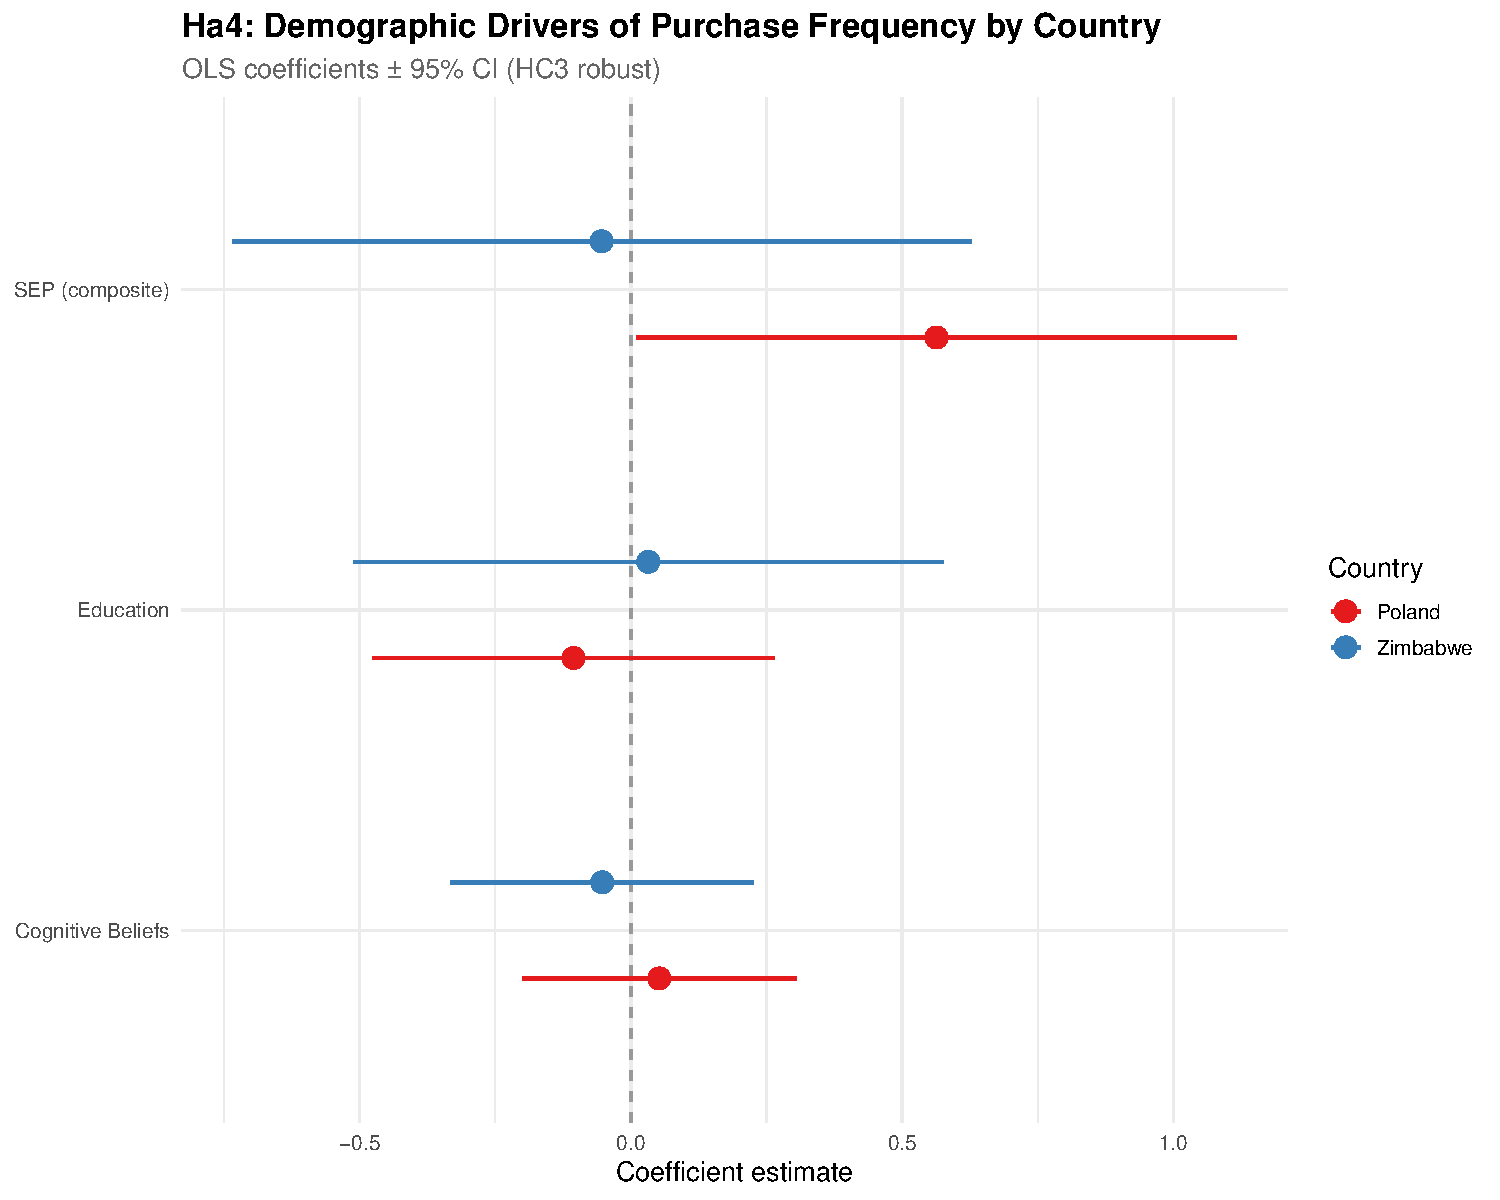
\includegraphics[keepaspectratio]{final_analysis_files/figure-pdf/unnamed-chunk-11-1.pdf}}
\end{center}

\begin{Shaded}
\begin{Highlighting}[]
\CommentTok{\# ggsave("Ha4\_country\_demographic\_drivers.png", p\_ha4,}
\CommentTok{\#        width = 9, height = 5, dpi = 300)}
\end{Highlighting}
\end{Shaded}

\subsection{Consolidated Models}\label{consolidated-models}

\begin{Shaded}
\begin{Highlighting}[]
\FunctionTok{modelsummary}\NormalTok{(}
  \FunctionTok{list}\NormalTok{(}
    \CommentTok{\# Ha1}
    \StringTok{"Aff \textasciitilde{} Cog"}        \OtherTok{=}\NormalTok{ bk2,}
    \StringTok{"PF \textasciitilde{} Cog + Aff"}   \OtherTok{=}\NormalTok{ bk3,}
    \CommentTok{\# Ha2}
    \StringTok{"PF \textasciitilde{} Cert"}        \OtherTok{=}\NormalTok{ bk2\_ha2,}
    \StringTok{"D2 \textasciitilde{} Cert + PF"}   \OtherTok{=}\NormalTok{ bk3\_ha2,}
    \CommentTok{\# Ha3}
    \StringTok{"Ha3 Base"}         \OtherTok{=}\NormalTok{ ha3\_base,}
    \StringTok{"Ha3 3{-}Way"}        \OtherTok{=}\NormalTok{ ha3\_3way,}
    \CommentTok{\# Ha4}
    \StringTok{"Ha4 Poland"}       \OtherTok{=}\NormalTok{ ols\_pol,}
    \StringTok{"Ha4 Zimbabwe"}     \OtherTok{=}\NormalTok{ ols\_zim}
\NormalTok{  ),}
  \AttributeTok{statistic =} \StringTok{"(\{std.error\}) [\{conf.low\}, \{conf.high\}]"}\NormalTok{,}
  \AttributeTok{stars     =} \FunctionTok{c}\NormalTok{(}\StringTok{"*"} \OtherTok{=}\NormalTok{ .}\DecValTok{10}\NormalTok{, }\StringTok{"**"} \OtherTok{=}\NormalTok{ .}\DecValTok{05}\NormalTok{, }\StringTok{"***"} \OtherTok{=}\NormalTok{ .}\DecValTok{01}\NormalTok{),}
  \AttributeTok{vcov      =} \StringTok{"HC3"}\NormalTok{,}
  \AttributeTok{notes     =} \StringTok{"HC3 heteroskedasticity{-}robust standard errors in parentheses; 95\% CIs in brackets."}\NormalTok{,}
  \AttributeTok{output    =} \StringTok{"Hypothesis\_Results\_Table.docx"}
\NormalTok{)}
\end{Highlighting}
\end{Shaded}





\end{document}
